\chapter{Introduction}
\label{ch:Intro}


%%%%%%%%%%%%%%%%%%%%%%%%%%%%%%%%%%%%%%%%%%%%%%%%%%


\section{Psoriasis and psoriatic arthritis}
%
Psoriasis and psoriatic arthritis (PsA) have been progressively identified as two different common complex disease entities. Psoriasis is a chronic inflammatory dermatose disease with episodes of relapse and remitance \parencite{Nestle2009}. On the other hand, PsA is a seronegative chronic inflammatory disease within the family of spondyloarthritis \parencite{Moll1973, Coates2016} that usually develops after the psoriasis skin manifestations\parencite{Villanova2016}. Psoriasis and PsA have shared and distinct clinical features, which are likely a reflection of the commonalities and differences in genetic loci contributing to disease development. It is important to understand those commonalities and differences at the physiological and genetic level in order to better understand the relevance of the genetic variability in the risk to develop psoriasis and PsA.

%(Variants in RUNX3 contribute to susceptibility to PsA, exhibiting further common ground with ankylosing spondylitis, PsA Immunochip)

\subsection{Epidemiology and global impact}
%
Psoriasis represents a serious global health problem that currently affects about 100 million people worldwide, including children and adults with no sex bias \parencite{Organization2016}. Although there is a very weak correlation with geographic latitude \parencite{Jacobson2011}, it has been reported to vary upon ethnicity. For example, psoriasis prevalence in adults is lower among African, African American and Asian (0.4-0.7\%) compared to American and Canadian (4.6 and 4.7\%, respectively) populations. In the UK, psoriasis prevalence ranges between 2-3\% and it affects approximately 1.8 million people \parencite{Perera2012}.

PsA prevalence in the general population ranges between 0.04-1.2\% \parencite{Perera2012}but it dramatically increases to 10-30\% within psoriasis cases \parencite{Gelfand2005,Reich2008} and evidences the association between the two diseases. Particularly, in the UK, 14\% of the psoriasis patients develop chronic inflammatory arthritis in the form of PsA at some point of the disease course \parencite{Ibrahim2009}. %Overall, data suggests an steady increase in both, psoriasis and PsA, prevalence over time \parencite{Springate2007,Organization2016}.

Although psoriasis can be developed at any age, onset of disease seems to have a bimodal distribution strongly influenced by the Human Leukocyte Antigen (HLA) Cw*06:02 (HLA-Cw6:02), an allele for one of the genes in the Major Histocompatibility Complex (MHC) I, involved in antigen presentation \parencite{Henseler1985} and the strongest genetic association with psoriasis and PsA risk \parencite(Ellinghaus2010, Strange2010, Stuart2010; Sun2010). The early-onset or Type I is characterised by development of disease around 16-22 and 30-39 years and a prevalence for HLA-C*06:02 (85.4\% of the cases). In contrasts, the late-onset or Type II group manifests disease between 50-60 years old and presents positive HLA-C*06:02 only in 14.6\% of the cases. %This classification based on the age of onset has also correlates with distinctive clinical clinical features including severity, relapse frequency and family history.

Psoriasis and PsA also represent an economical burden for the countries' economies due to treatment and associated morbidity. For example, in the UK treatment and management of psoriasis in 2015 ranged between £4,000 to £14,000, before and after requirements of biological therapy, respectively \parencite{Burgos-Pol2016} and the costs are even greater for PsA \parencite{Poole2010}.


\subsection{Psoriasis and inflammatory dermatoses}
%

The group of inflammatory dermatoses affects up to 70\% of the population, regardless age and geographic location \parencite{ICD-10}, and it represents the 4$^{th}$ leading cause of nonfatal burden \parencite{Roderick2014}. The skin is the biggest organ in the human body constituting an effective barrier between the environment and the internal organs. The most external layer, the epidermis, plays a relevant role in the innate and adaptive immunity \parencite{Proksch2008} and its alterations due to exogenous or endogenous factors can lead to development of inflammatory dermatose conditions, such as psoriasis, atopic dermatitis (AD) or cutaneous lupus erythematosus (CLE) \parencite{Johnson-Huang,2009}. Lesions in psoriasis can be non-pustular and pustular which reflects the heterogeneity in the type, location and severity of the disease and impairs the clinical classification \parencite{Perera2012}. As a result, several phenotypes of psoriasis including vulgaris, guttate, pustular, erythroderma and nail pitting have been defined and it is under debate whether some of those should be considered a different disease entity \parencite{Marrakchi2011}.


\subsection{PsA and spondyloarthropaties}
%
PsA belong to the family known as spondylarthropaties (SpA) which also includes other subtypes such as ankylosing spondylitis (AS), reactive arthritis (ReA), idiopathic inflammatory bowel disease (IBD) and undifferentiated SpA \parencite{Baeten2013}. All SpA subtypes are characterised by structural damage (bone formation and erosion) as well as inflammation of joints and extraarticular sites such as eyes, gut and skin. Additional SpA criteria have led to a reduced classification of SpA into axial and peripheral SpA based on the affected joint (spine/sacroilicac or peripheral) and the presence of extraarticular features \parencite{Runwaleit2001, Runwaleit2001}. Studies in human families and rat models with HLA-B27 positive status have shown manifestation of different SpA forms, such as psoriasis and IBD, within a single family or individual \parencite{Hammer1990,Said-Nahal2000 \parencite}. These observations support the hypothesis that SpA subtypes may be a single multifaceted condition with shared genetic, immunophatological and structural features and dynamic phenotypes \parencite{Baeten2013}. Conversely, some studies suggest that multiple genetic factors may be involved in the determination of the axial and peripheral arthritis and partially explain the immunopathological differences between the two \parencite{Porcher2005, Appel2011, Noordenbos2012}.

As a phenotype, PsA can be further subdivided in five clinical groups based on Moll and Wright criteria: distal, destructive, symmetric, asymmetric and spinal \parencite{Moll1973}. These subclasses mainly differed upon the location, number and distribution of the affected joints. Later studies have questioned this method of classification due overlapping of the different subsets and lack of  inclusion of dactylitis (diffuse swelling of a digit) a distinctive feature of PsA \parencite{Reich2009}. This phenotypic heterogeneity increases the difficulty in the design and achievement of meaningful outcomes from clinical studies.



\section{Pathophysiology of psoriasis and psoriatic arthritis}

\subsection{Clinical presentation and diagnosis}
%
Approximately 90\% of all psoriasis cases are plaque psoriasis vulgaris that manifests with raising well demarcated plaques, erythema and scaling. The thickening (acanthosis) and vascularisation of the epidermis leads to the plaques formation \parencite{Perera2012} that can vary in size and distribution, being the most common the elbows, knees and scalp \parencite{Griffiths2007}. The second most common type is psoriasis guttate (10\% of all cases) characterised by acute onset of small droplike papules usually in the trunk and proximal extremities \parencite{Vence2015}. Type I psoriasis commonly appears in the form of guttate lesions after bacterial infection whilst type II involves spontaneous chronic plaques \parencite{Perera2012}. %Unlike pustular psoriasis, the least prevalent phenotype, vulgaris and guttate forms are not life threatening \parencite{Moura2015}.  

In PsA the most common manifestation is the symmetric/polyarticular (more than 50\%) followed by the asymmetric/oligoarticular (around 30\%) PsA, that affects single or few distal interphalangeal or phalangeal joints \parencite{Reich2009, McGonagle2011}. The psoriatic lesions precede joint inflammation in approximately 60-70\% of the cases\parencite{Gladman2005, McGonagle,2011}. Particularly, nail, scalp and intergluteal lesions constitute a predictive biomarker for development of joint inflammation \parencite{Moll1976,Griffiths2007,McGonagle,2011}. This reinforces the need of appropriate coordination between dermatologists and rheumatologists for an early diagnostic and treatment that could prevent functional joint disability.

Several comorbidities have been associated with psoriasis and PsA, with comparatively greater prevalence in PsA. For example, intraocular inflammation known as uveitis affects 8\% of PsA patients compared to 2\% of the psoriasis ones \parencite{Husted2011, Oliveira2015}. Other comorbidities include inflammatory bowel disease(IBD), cardiovascular disease (CVD) \parencite{Gelfand2006}, type II diabetes (T2D) \parencite{Saphiro2007} and metabolic syndrome \parencite{Cohrn20017}. %Psoriasis and PsA have also important implication in the mental health of the patients and they are associated with an increased prevalence of depression and suicidal ideation \parencite{Sampogna2012}.

The diagnosis of psoriasis and PsA is mainly based in clinical assessment since there is a lack of appropriate biomarkers at early stages of disease \parencite{Villanova2013}. Evaluating the severity of psoriasis skin lesions remains challenging and different measures have been implemented. The Psoriasis Area and Severity Index (PASI) \parencite{Fredriksson1978} is the most widely used in research and drug trials \parencite{Finlay2005}. This test quantifies lesional burden weighted by body part based on the amount of affected body surface area and the degree of severity of erythema, induration and scale (Table \ref{tab:PASI}). Disease is considered mild for PASI<7 and it is classified as moderate-to-severe for PASI>7-12, depending on the study \parencite{Finlay2005, Schmitt2005,add ref from cell types}.

To evaluate PsA, analysis of performance of the previously mentioned Moll and Wright criteria together with additional ones led to the configuration of the Classification Criteria for Psoriatic Arthritis (CASPAR) \parencite {Taylor2006}, the most widely used. It requires the patient displaying inflammatory arthritis, enthesitis, and/or spondylitis and three points from a list of associated elements (Table \ref{tab:CASPAR}) . Another composite measure commonly used to evaluate treatment efficacy for PsA is the PsA Response Criteria (PsARC) based on the number of tender joints (TJC) and swollen joints (SJC) over 68 and 66, respectively, as well as a physician global assessment based on a short questionnaire \parencite{Philipp2011,Clegg1996}.


\begin{table}[htbp]
\setlength{\tabcolsep}{20pt}
\renewcommand{\arraystretch}{1.5}
\begin{tabular}{@{} c c}
\textbf{PASI} & \textbf{description} \\
\midrule
\midrule
Body location  & Head and neck, upper limbs, trunk and lower limbs\\
Feature        & Redness, thickness and scaling \\
Severity scale & Absent, mild, moderate, severe or very severe \\
Affected area (\%)  & 0, 1-9, 10-29, 30-49, 50-69, 70-89 or 90-100 \\
\bottomrule
\end{tabular}
\medskip %gap
\caption[Variables and scoring used in the Psoriasis Area and Severity Index (PASI)]{\textbf{For each of the four body locations the test quantifies the percentage of affected area and the severity of three intensity features: redness, thickness and scaling.}}
\label{tab:PASI}
\end{table}
\bigskip %bigger space




\begin{landscape}
\begin{table}[ht]
%\renewcommand{\arraystretch}{1.5}
\begin{tabular}{cccccccc}
		\multicolumn{2}{}{\textbf{CASPAR: a patient must have inflammatory articular disease (joint, spine, or enthesial) }} \\
		\multicolumn{2}{}{\textbf{ with three points from five categories}} \\
		\midrule
		\midrule
    \multirow{3}{*}{Psoriasis} & a. Current skin or scalp disease \\ & b. History of psoriasis \\ & c. Family history of psoriasis \\
    \hline
		\multirow{1}{*}{Psoriatic nail involvement} & Typical psoriatic nail distrophy\\ 
		\hline
    \multirow{1}{*}{A negative test for RF} & Using preferrably by enzyme-linked immunosorbent assay (EMSA)\\ 
    \hline
    \multirow{2}{*}{Dactylitis} & a. Swelling of an entire finger \\ & b. History of dactylitis\\ 
    \hline
		\multirow{1}{*}{Radiologic evidence of juxtaarticular new bone formation} & Ossification near joint margins\\ 
		\hline
    \bottomrule
		\end{tabular}
		\medskip %gap
		\caption[CASPAR criteria for diagnosis of PsA]{\textbf{xxxx}}
\label{tab:CASPAR}
\end{table}
\end{landscape}
\bigskip %bigger space


%PsARC is composed of four measures,including: 1) patient global assessment of disease activity (improvement of 1 on a 5 point Likert scale is required for a response), 2) physician global assessment of disease activity (improvement of 1 on a 5 point Likert scale is required for  esponse), 3) joint pain (reduction of 30% or more in total score, assessing either 68 or 78 joints, using a 4 point scale is required for a response), and 4) joint swelling (reduction of 30% or more in total score, assessing either 66 or 76 joints using a 4 point scoring scale, is required for a response).




\subsection{Aetiology of psoriasis and PsA}

Psoriasis and PsA are complex chronic inflammatory diseases where a dysregulated immune response initiates as result of genetic predisposition and exposure to a particular environmental trigger (Figure\ref{fig:PSO_aetiology_diagram}). One of the greater controversies has been characterising the origin of the pathologies as well as the connection between skin and joint inflammation. Particularly, for psoriasis it remains unclear whether disruption of the skin triggers activation of the immune response or viceversa.

%\begin{figure}[H]
%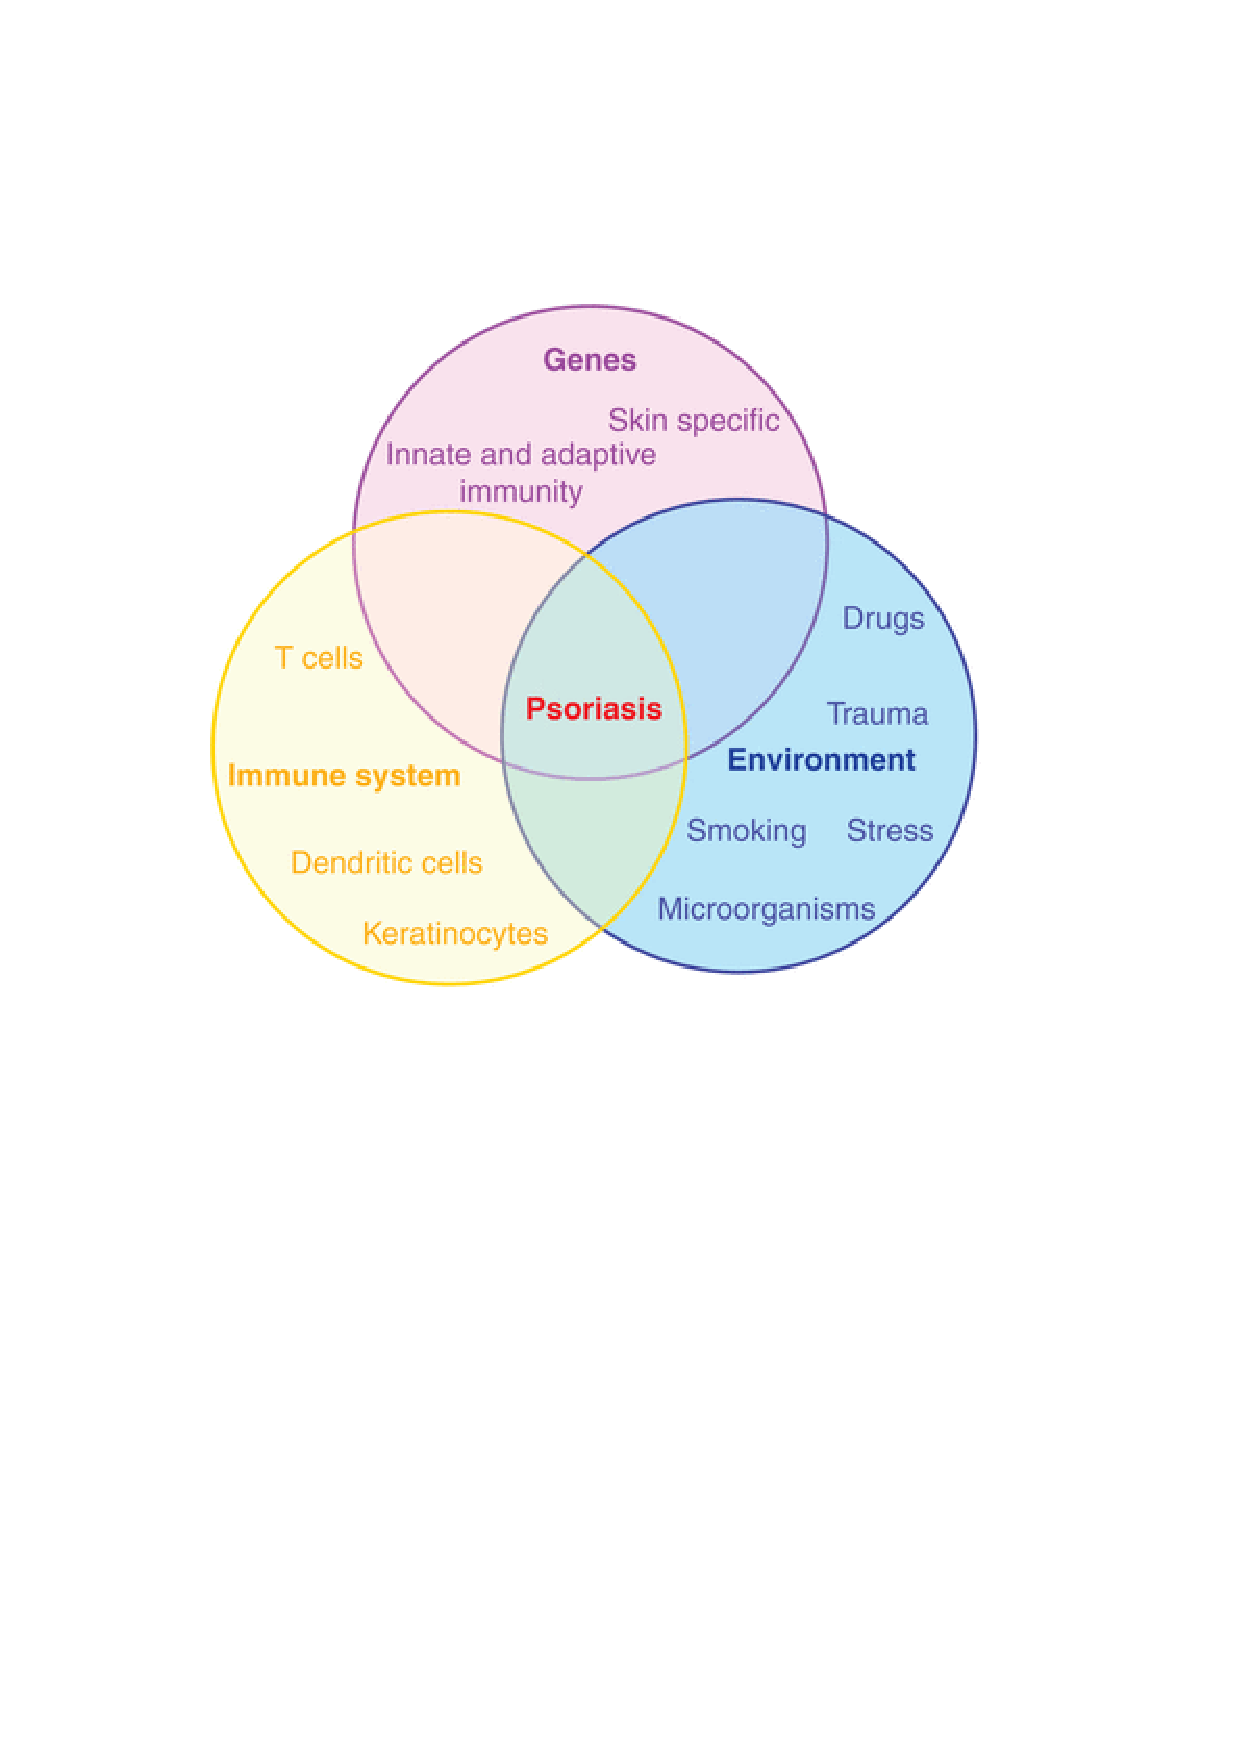
\includegraphics[width=\textwidth]{./Introduction/pdfs/PSO_aetiology_diagram_Di_Meglio_et_al_2014.pdf}
%\caption[Main factors involved in psoriasis disease aetiology]{\textbf{Figure adapted from \parencite{Meglio2014}}}
%\label{fig:PSO_aetiology_diagram}
%\end{figure}


\subsubsection*{Histopathological alterations in skin and joints}

The epidermis is the most external structure of the skin and it is formed by approximately 90\% keratinocytes (KC) organised in a layer structure that self-renews in a time dependent manner from the bottom to the surface \parencite{Wikramanayake2014}. As the KC differentiate they undergo changes in morphology, replication ability and keratin composition of their intracellular matrix. In the context of psoriasis impaired epidermis cell renewal leads histological alterations and development of the psoriatic lesions. KC undergo upregulation in the proliferation rate (hyperplasia) that causes aberrant cell differentiation (parakeratosis) (ref) thickening of the epidermis and the subsequent scale formation (ref). Concomitantly, inflammation causes immune cell infiltration and hypervascularisation of the lesion driven by upregulation in the expression of angiogenic factors and activation of the endothelium \parencite{Perera2012}. 

In PsA, joint affection usually follows skin lesions and it involves a wide range of histological changes in the joints, particularly bone remodeling \parencite{Haddad2013}. One of the most common structural changes is the arthritis caused by the swelling and inflammation of the joints \parencite{Schett2011}. As result of this inflammation, alterations in bone remodeling leads to osteolysis with subsequent bone resorption and erosion at the affected joints \parencite{Mensah2017}. This phenomenon is particularly relevant in arthritis mutilans or chronic absortive arthritis, one of the most severe forms of PsA \parencite{Haddad2013}. Bone erosion is also the main histopathological process driving dactylatis, where bone lysis resolves in shortening of the digits \parencite{Gladman2005}. On the other hand, 35\% of the PsA patients undergo inflammation of the connective tissue at the insertion of tendons or ligaments, phenomenon known as enthesitis \parencite{McGonagle2011,Polachek2017}. Overtime, this causes debilitating structural changes due to formation of bony spurs along the insertion sites\parencite{Schett2011}.


\subsubsection*{Dysregulation of the innate and adaptive immune response}
%link to the histological changes
The dysregulated  immune response in psoriasis and PSA is the result of the interaction between innate and adaptive immune cells (ref section) resulting in feedback loops involving a complex cytokine milieu. Among the most relevant cytokines of the innate immunity involved in disease initiation are IFN-$\alpha$ and IFN-$\gamma$ \parencite{Leanne2009}. They are mainly produced by circulating plasmacytoid DC (pDC) and myeloid DC (mDC), respectively, upon activation by KC pro-inflammatory cytokines \parencite{Perera2012}. Both are upregulated at the mRNA level in the lesional skin and contribute to lymphocyte recruitment and maintenance of DC activation \parencite{Schmid1994}. 

Another key cytokine in this dysregulated inflammatory response is TNF-$\alpha$ which has a prominent role in bone turnover and bone remodeling in PsA \parencite{Mensah2008}. It is produced by activated KC, mast cells but also by adaptive immune cells types, including infiltrated T helper(Th) 1 and Th-17 cells infiltrated in the psoriatic lesion and PsA inflamed joints \parencite{Perera2012} and it induces activation of nuclear factor kappa-light-chain-enhancer of activated B cells (NF-$\kapa$B) signaling pathways (ref). It also activates several kinase signaling pathways as well as cell death programs (ref). In the context of inflammation, NF-$\kapa$B represents a master transcriptional regulator of both, the innate and adaptive immune system that induces expression of proinflammatory cytokines, antiapoptotic genes and genes involved in chronic inflammation maintenance (ref). The importance of this transcription factor (TF) in psoriasis and PsA pathogenesis is reflected by the association with disease of several genetic variants in some of the negative regulators of its proinflammatory activity, including NF-$\kapa$B inhibitor alpha \textit{NFKBIA} and TNF receptor-associated factor 3 interacting protein 2 \textit{TRAF3IP2} (ref).
 
Interleukin-23 (IL23) and Th17 axis represents a key loop for the maintenance of psoriasis and PsA inflammatory response and a very important link between innate and adaptive immunity. IL-23 is an innate regulatory cytokine, mainly produced by mDC and macrophages homing the inflamed skin and it binds to the IL-23 receptor (IL-23R), which expression is upregulated in the DC and T cells of the lesion and in circulating Th cells (ref). In psoriasis, IL-23 is the mediator for the pathogenic loop between activated KC and T cells (ref). Both IL-23 and IL-23R present protective and pathogenic genetic variants associated with psoriasis and PsA risk (ref). The activation of the IL-23 pathway leads importantly to increased IL-17 production through NF-\kappaB activation by \textit{TRAF3IP2} (ref). IL17 favors maintenance of the adaptive immune mediated Th17 response through recruitment and activation of neutrophils, induction of proinflammatory cytokines including IL-1\beta and IL-6 and also perpetuation of KC activation (ref) (https://www.ncbi.nlm.nih.gov/pmc/articles/PMC3580541/). % add info
More recently, interleukin 22 (IL-22) has arisen as another of the key cytokines in mediating the dysregulated cross talk between the innate and adaptive immune response. IL22 levels are increased in the psoriatic lesions and serum of patients and it is mainly produced by a subset of CD4$^+$ cells known as Th22 (ref). It mediates some of the histological changes in skin as well as AMP production by KC (ref).

% Maybe a paragraph to connect skin and joint affection Identical T cell clonality between skin and synovium https://ac.els-cdn.com/S0198885999000348/1-s2.0-S0198885999000348-main.pdf?_tid=5efa7316-fde5-11e7-8091-00000aacb360&acdnat=1516454913_dd20efb867f822d68d8b09873601e8ad

\subsubsection*{Environmental factors and disease}

Several environmental triggers are known to be associated with increased risk and worsening of psoriasis and PsA development. A wide range of drugs including antidepressant, antihypertensive and anticytokine therapies have been clinically associated with initiation, exacerbation and worsening of psoriasis \parencite{Kim2010}. Infectious agents such streptococcal throat infection have likewise been associated with development of type I psoriasis \parencite{Gudjonsson2003,Valdimarsson2009, Diluvio2006}. Consistently with other chronic inflammatory disease such as IBD and AS, recent studies have also observed perturbation in the composition of the gut and skin microbiota in psoriasis and PsA patients \parencite{Eppinga2014}. On the other hand, physical trauma, including tattoos, surgical incisions and mechanical stress can trigger the appearance of lesions in psoriatic uninvolved skin as well as joint inflammation in digits \parencite {Weiss2002,Nestle2009}. Lastly, as for most of the complex diseases, behavioral factors including smoking, alcohol and stress have been linked to psoriasis and PsA without a clear conclusion of their involvement in triggering disease \parencite{Meglio2014}.

\subsection{Cell types involved in psoriasis and PsA pathogenesis}
%Global report on psoriasis, 2016

Identifying the most relevant cell types contributing to psoriasis and PsA pathogenesis remains challenging. There has been a reinterpretation of both phenotypes that understands them as dynamic and continuous processes where different cell types became predominantly important at different stages of the pathology. 

KC are one of the most relevant cell type at early stages of psoriasis pathogenesis, which is reinforced by the genetic association between skin specific genes from the late cornified envelope (LCE) family and psoriasis \parencite{Tsoi2012}. Several studies have shown the role of KC as immune sentinels through MHC-II antigen presentation and production of antimicrobial peptides (AMP), cytokines and chemokines \parencite{Black2007}. There is evidence of complex formation between the cationic AMP LL-37 and self-DNA/RNA released by KC upon damaged triggered by environmental factors \parencite{Lande2007}. This complex acts as an antigen for activation of the skin-resident DC \parencite{Nestle2005} and that initiate and perpetuates the skin inflammatory response through secretion of pro-inflammatory cytokines, importantly IL-1, IL-6 and TNF-$\alpha$ \parencite{Feldmeyer2007, Arend2008, Nestle2009}. Studies in mouse models have also shown development of psoriatic lesions in immunodeficient mice upon human xenotransplant of psoriasis skin\parencite{Boyman2004}. Overall, these findings would support the hypothesis attributing the initiation of the chronic inflammatory response in psoriasis as the consequence of the epidermis dysfunction \parencyte{Proskch2008}. 

mDC and pDC are professional APC also considered important innate immune cells in disease initiation through T cell activation and subsequent triggering of the adaptive immune response \parencite{Mahil2016}. %The relevance of antigen presentation in disease has been highlighted at the cellular \parencite{Rusell1972, Tiilikainen1980} and also at the genetic level with the psoriasis and PsA GWAS association of HLA-Cw*06:02 and ERAP1 \parencite{Strange2010}, which encodes for an aminopeptidase involved in the trimming of peptide antigens.
pDC are circulating cells absent in healthy skin that infiltrate into the lesional and uninvolved dermis of psoriasis patients and get activated by the aforementioned KC self-DNA and LL-37 complex through Toll-like Receptor (TLR)-9 \parencite{Nestle2005, Lande2007}. In contrast, quiescent mDC are epidermal resident cells and upon secretion of IFN-$\alpha$ by pDC a 30-fold increase of mature mDC is observed in lesional skin but not in uninvolved or healthy tissue (ref). Different mDC subpopulation mediate the Th1 and Th17 response as well perpetuation of KC activation through IL-23 production (ref). Studies in immunodeficient psoriasis mice models have shown that blockage of downstream  IFN-$\alpha$ signaling or its production by pDC failed to induce T cell activation and onset of psoriasis \parencite{Nestle2005}. 

Neutrophils are also though to be closely involved in disease initiation through their ability to form neutrophil extracellular traps (NET)that contain host DNA and LL-37 \parencite{Hu2016}. There is evidence of increased NET formation in peripheral blood and lesional skin of psoriasis patients and they seem to be contributing to pDC and CD4$^+$ T activation \parencite{Hu2016}. Neutrophils have also been identified in recent studies as one of the main sources of IL-17 production in the skin lesions \parencite{Lin2011} and they also release a wide range of proteases which some induce KC proliferation \parencite{Mahil2006}.

In the context of the innate immunity, the involvement of monocytes and macrophages in psoriasis and PsA has not been extensively studied. Resident macrophages in the healthy dermis undergo a 3-fold increase upon skin lesion and they are involved in disease development through TNF$\alpha$ production \parencite{Perera2012, Mahil2016}. Similarly, mice models for chronic psoriasiform skin inflammation have shown macrophage migration into the affected skin and TNF-$\alpha$ production for maintenance of the skin lesions \parencite{Stratis2006, Wang2006}. Some studies using isolated monocytes from psoriasis patients PBMC  have shown greater phagocytic and bactericidal activity compare to those from healthy individuals \parencite{Bar-Eli1979}. Later studies have also shown increased circulating intermediate monocytes (CD14$^{+}$ high CD16$^{+}$ high) and monocyte aggregation in psoriasis patients causing enhanced platelet activation and angiogenesis \parencite {Golden2015}. In PsA, synovial membranes levels of monocytes/macrophage metalloproteinases which mediate bone erosion through differentiation into osteoclasts are comparable to those found in RA joints \parencite{Hitchon2002}. Overall, these observations highlight the systemic aspects of both pathologies. 

%HLA-Cw*06:02 can be recognised by the inhibitory receptor KIR2DL1 and the activatory receptor KIR2DS1.  Some studies have shown KIR2DS1 was present in 85\% of the patients but only in 51\% of the controls
%NK cells are important regulators of immune responses \parencite{Luszczek2004}. Their function extends beyond killing of infected or transformed cells. Interactions with dendritic cells, macrophages, and fetal trophoblast cells can regulate NK cell activity by influencing cytokine production, cytotoxicity and stimulation of T helper-1 responses. 
%
%


Historically, T lymphocytes have been considered one of the most relevant cell types in initiation and maintenance of psoriasis and PsA and its role is also supported by genetic findings. Report cases in humans have demonstrated that bone marrow transplantation can initiate or terminate psoriasis \parencite{Eedy1990, Gardembas1990}. The percentage of circulating T cells in psoriasis have shown reduced number of T cells in moderate-to-severe and severe psoriasis patients but increased percentage of the memory populations CD4$^{+}$CD45RO$^{+}$ and CD8$^{+}$CD45RO$^{+}$ when compared to milder phenotypes and healthy controls \parencite{Lecewicz-Toruń2001,Langewouters2008}. There is still controversy regarding the total CD4$^+$ and CD8$^{+}$ abundance and CD4$^{+}$/CD8$^{+}$ ratios in PBMC, which may be due to the phenotype heterogeneity of psoriasis patients in the different studies \parencite{Lecewicz-Toruń2001,Cameron2003,Langewouters2008}. In PsA, no differences  abundance of circulating T cells have been identified compared to healthy individuals \parencite{Costello1999}.

In healthy skin, CD4$^{+}$ and CD8$^{+}$ are found in the dermis and epidermis, respectively \parencite{Clark2006,Perera2012} and an increase in activated memory CD4$^{+}$CD45RO$^{+}$and CD8$^{+}$CD45RO$^{+}$ can be detected as soon as 3 days after lesion appearance \parencite{Clark2006}, highlighting the importance of the memory population. \textit{In vivo} studies conducted in mice by Boyman and colleagues showed that development of psoriasis following engrafted human pre-lesional skin was dependent of local T cell proliferation without injection of additional factors \parencite{Boyle2013}, supporting that recruitment of circulating T cells may be restricted to the priming event and it is minimal afterward \parencite{Perera2012}. The relative importance of CD4$^{+}$versus CD8$^{+}$ in psoriasis initiation has been tested immunodeficient mice with pre-lesional skin xenografts suggesting a model where CD4$^{+}$ but not CD8$^{+}$ T cells where required for the progression of uninvolved to lesional skin in mice \parencite{Nickoloff1999}. Interestingly, injection of CD4$^{+}$ activated cells was followed by an increase in activated resident CD8$^{+}$ T cells expressing the acute activation marker CD69 which suggests that skin CD4$^{+}$ cells drive activation of resident T cells and that the activated CD8$^{+}$ resident population would act as the main effector cells. In PsA, CD4$^{+}$ are significantly more abundant than CD8$^{+}$ cells in synovial tissues \parencite{Diani2015}. However, among the CD8$^{+}$ population the memory cells are prevalent in the SF and they are significantly increased when compared to controls \parencite{Costello1999}. The contribution of regulatory T (Treg) cells have also been investigated with controversial outcomes regarding relative abundance and impaired function in both pathologies \parencite{Perera2012}. 

Based on the T cells cytokine profile, psoriasis and PsA has been demonstrated to be a type 1 Th/Tc disease, where activation of na\"{i}ive CD4$^{+}$ and CD8$^{+}$ cells is driven by IL-12 and IFN-$\gamma$ \parencite{Austin1999,Perera2012}. Later studies have also identified additional T cells subsets including Th-17/Tc-17 and Th-22/Tc-22, characterised for the high production of IL-17 and IL-22, respectively, two cytokines very relevant for perpetuation of the inflammatory response \parencite{Mahil2016}.  The importance of Th17 cells and IL-17 production has been assessed in skin, joints and blood, where elevated IL-17 and also IL-23 mRNA and protein levels have been found in psoriasis and PsA patients compared to controls \parencite{Cai2012, Dolcino2015}. It has been shown that the predominant CD8$^{+}$ populations in the SF are also IL-17 producers and their abundance correlates with markers of inflammation and structural changes in the joint \parencite{Menon2014}. This finding is in line with observations in skin and it suggests a prominent role of CD8$^{+}$ IL-17 producing cells in the different stages of both pathologies. Understanding the importance of IL-17 has also led to the discovery of other immune cells producing this pivotal cytokine, including innate immune lymphoid (ILC) cells and $\gamma$$\delta$ T cells which have also started to be investigated in the context of psoriasis and PsA pathophysiology and treatment \parencite{Meglio2014,Leijten2015}. IL-17 producing cell have also been hypothesised to be responsible for the link between skin and joint lesions. Although the precise mechanisms for transition between psoriasis and PsA is unknown, studies using psoriasis and RA mice models have shown that skin lesions facilitate arthritis and joint inflammation % \parencite{}. The presence of IL-17 producer cells in inflamed skin located nearby the enthesis of joints under physical stress could trigger the development of PsA.

\begin{figure}[H]
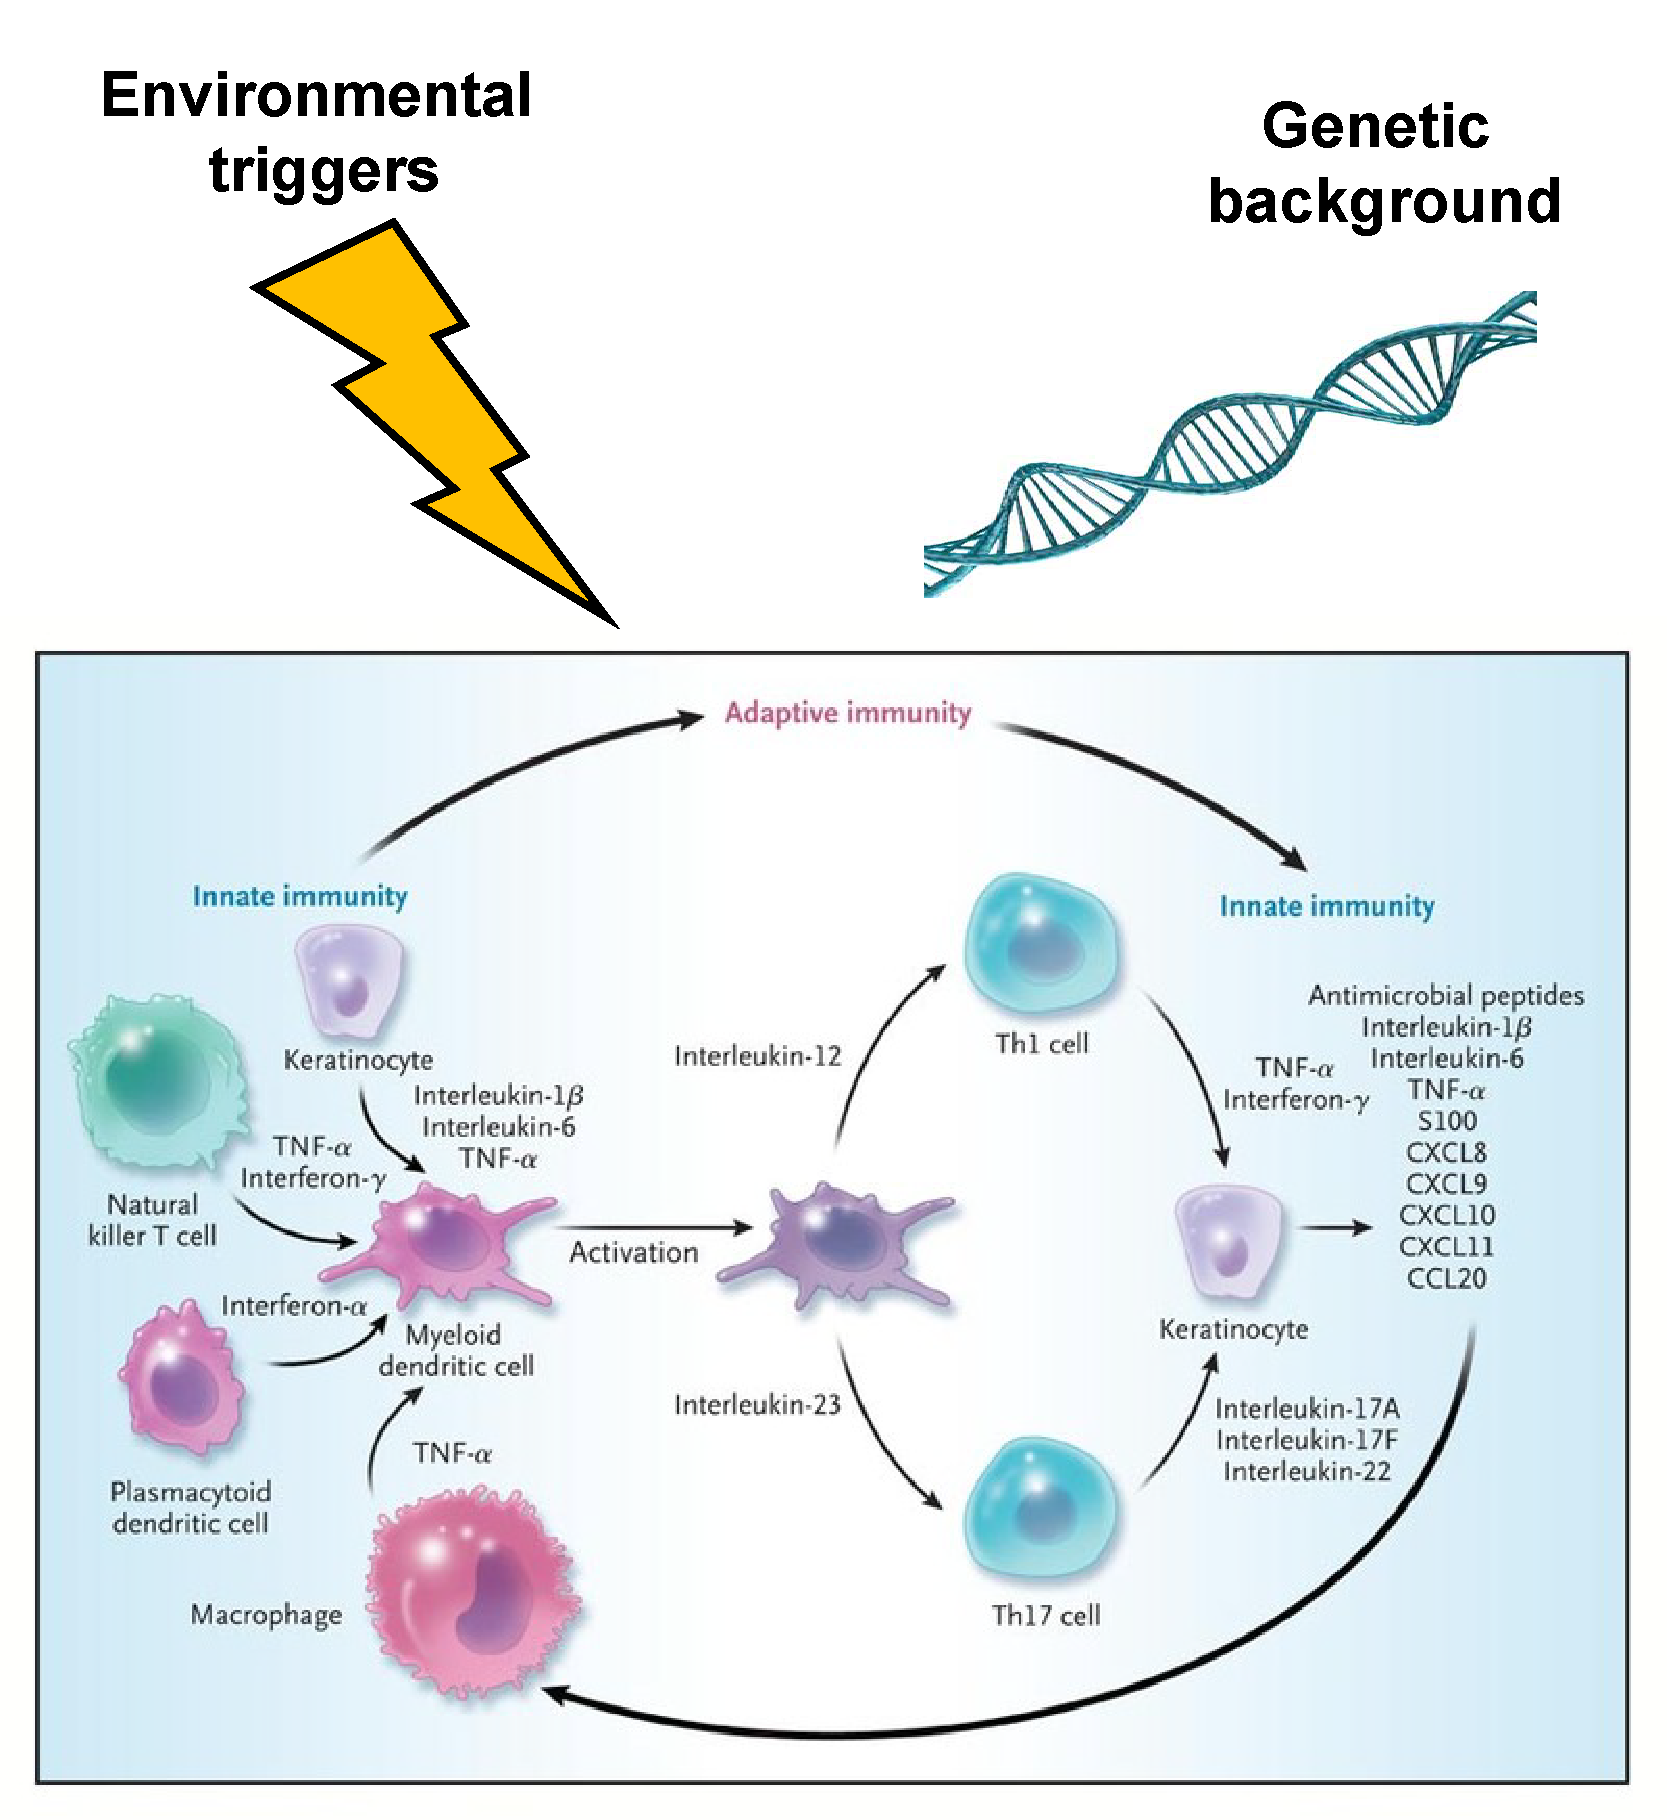
\includegraphics[width=\textwidth]{./Introduction/pdfs/PSO_adaptive_innate_immune_system_crosstalk.pdf}
\caption[Crosstalk between innate and adaptive immunity in psoriasis]{\textbf{Figure adapted from \parencite{Nestle2009}}}
\label{fig:PSO_immune_system_diagram}
\end{figure}

\subsection{Therapeutic intervention and prognosis}

Currently, there is no cure for either psoriasis or PsA and the different treatments available are focused in managing symptoms. The approach to treat them are usually dependent on the disease severity. Cases of mild-to-moderate psoriasis are usually managed with topical therapies for which corticosteroids and emollients are the most commonly used and affordable ones \parencite{Menter2009}. %Some of the corticosteroids are approved only for short term treatments as side effects have been reported at a local and systemic level \parencite {Menter2009}. 
In psoriasis, other topical treatments are used in combination with corticosteroids such ultra violet (UV) light therapy and vitamin D analogues, which inhibit KC proliferation, stimulate KC differentiation and inhibits T cell proliferation \parencite{Rizova2001}. For PsA patients presenting swelling of two or less joints, intra-articular injection of glucocorticosteroids together with joint aspiration have shown to reduce pain and inflammation as a short-time measure \parencite{Coates2016}. 

Treatment of most forms of PsA and more moderate-to-severe psoriasis require the use of a broad range of systemic therapies. For mild cases of PsA nonsteroidal anti-inflammatory drug (NSAID) are the most commonly used to help controlling the mild inflammatory symptoms \parencite{Coates2016}. For more severe forms of PsA, disease-modifying antirheumatic drugs (DMARDs) including the an antagonist of folic acid methotrexate (MTX) and the phosphodiesterase 4 inhibitor apremilast are used with immunosupressive effects on activated T cells and cytokine production, respectively \parencite{Schmitt2014, Gossec2016, Keating2017,Polachek2017}. Biologic systemic agents are the most specific for the treatment of severe psoriasis and PsA. They are cell-based molecular species that modulate the immune response in a physiological manner \parencite{Perera2012}. Among the biologic agents targeting cytokines, TNF$\alpha$ inhibitors (TNFi) have been broadly used for the past five decades to treat both, psoriasis and PsA due to the relevance of TNF$\alpha$ in disease. Three TNFi have been approved for the treatment of psoriasis: etanercept, infliximab and adalimumab \parencite{Ahil2016}. In addition to those, certolizumab pegol and golimumab are also used in the management of PsA and other rheumatoid diseases \parencite{Coates2016b}. All the TNFi are antibody-based agents but etanercep, which is a soluble receptor, and they show differences in the frequency and via of administration \parencite{Mease2000}. Although TNF-$\alpha$ blockade is one of the most effective treatments, some patients experience common side effects such as increased risk of infection, reactivation of latent infections, demyelinating disease and induced pustular psoriasis have been identified \parencite{Nickoloff2004}. Between 20 to 50\% of the patients fail to respond to the first TNFi, due to side-effects or tolerance, and they require switching to a second or third one \parencite{Abramson2016}. New biologic therapies have been developed to target other key cytokines in the pathogenesis of PsA and psoriasis, such as IL-12 and IL-23 (ustekinumab) or  IL-17 (secukinumab and ixekizumab) \parencite{Mahil2016}. These new biologics represent a substantial benefit for treating patients and they are routinely administered to individuals failing to respond after a switch to a second TNFi \parencite{Coates2016b}.
% Bispecific antibodies
 

\section{Genetics of psoriasis and psoriatic arthritis}

As complex diseases, the risk to develop psoriasis and PsA is not only influenced by the surrounding environmental conditions but also by the genetic background of each individual. Determining the magnitude of contribution of the genetic factors in the development of these disease and identifying the exact genes or regions involved in the predisposition to psoriasis and PsA remains challenging. 


\subsection{Heritability}

Several studies have shown a trend towrads the increase of psoriasis and PsA prevalence over the last 30 years in different countries \parencite{Organization2016}. This importantly reflects changes in life style habits and it highlights the need to better understand the genetic factors that predispose to disease upon interaction with environmental stresses.

The contribution of genetics in the development of psoriasis has also been demonstrated in several twins studies. The concordance of psoriasis has been shown to be greater in monozygotic (33-55\%) compared to dizyogtic (13-21\%) twins with some variation between studies and populations, estimating an 80\% of heritability in this condition \parencite{Faber1974, Duffy1993, Pendersen2008}. For PsA, similar concordance between mono- and di- zygotic twins has been shown, probably due to lack of statistical power and appropriate diagnosis \parencite{Pendersen2008}. In the general population, approximately 40\% of the patients with psoriasis or PsA have family history in first degree relatives \parencite{Gladman1986}. Interestingly, the recurrence in first-degree relatives ha been shown to be greater in PsA (40) compared to psoriasis (8) in a study in Icelandic population \parencite{Chandran2009}. This could suggest differences in the heritability between the two phenotypes and maybe an stronger genetic contribution in PsA.

\subsection{Non-GWAS and linkage studies}
Different approaches have been undertaken to uncover the genetic variability contributing to the predisposition to psoriasis and PsA. The appearance of next generation sequencing (NGS) techniques and the progressive reduction of cost has allowed to move from candidate genes studies looking at the genetic variability at particular locus to a genome-wide approach.

The study of psoriasis and PsA genetics architecture started with linkage analysis in family pedigrees with autosomal dominant condition to try to . The use of this approach yielded nine psoriasis susceptibility loci (PSORS1-9) \parencite{Capon2017} with the strongest association in PSORS1 \parencite{International2003}. PSORS1 lies within chromosome 6p21.3 and its identification by linkage analysis confirmed the association previously identified in serological studies between psoriasis susceptibility and the MHC I \parencite{Rusell1972, Tiilikainen1980}. Importantly, Mendelian forms of disease with rare highly penetrant mutations have been identified in family studies for two genes within PSORS2 (17q25): zinc finger protein 750 (\textit{ZNF750}) \parencite{Tomfohrde1994} and caspase domain family member 14 (\textit{CARD14}) \parencite{Jordan2012}. Rare gain of function and \textit{de novo} mutations and also common variants in \textit{CARD14} have been identified in psoriasis and PsA patients, suggesting an important role of the genetic variation in this gene for Mendelian and multi-factorial forms of disease \parencite {Jordan2012, Tsoi2012}. In PsA, a region close to the psoriasis PSORS8 was also identified \parencite{Karason2003}. Nevertheless, the ability of independent studies to only reproduce PSOR1, 2 and 4, highlighted the limitations of the linkage studies to understand the genetics of complex diseases \parencite{Capon2017}. Gene based studies in psoriasis and PsA have also identified the relevance of genetic variability in the activating killer immunoglobulin receptors 2DS1 (KIR2DS1) \parencite{Łuszczek2004, Williams2005}, similarly to AS and RA \parencite{Carter2007, Yen2001}. This receptor is expressed on NK and NK T cells and mainly triggered by HLA-Cw*06:02. Similarly, specific association with PsA but not psoriasis was found for microsatellites and promoter polymorphisms in TNF-$\alpha$ \parencite{H\"{o}hler2002}. 



\subsection{Genome-wide association studies}
The technological advances experienced in sequencing and genotyping has allowed to implement association studies at a genome-wide scale. The genome-wide association studies (GWAS) have benefit from the understanding of common (frequency ${>}$1\%) single base-pair changes know as single nucleotide polymorphisms (SNPs) in different populations through whole genome sequencing (WGS) projects such as HapMap \parencite{The international HapMaP Consortium} project and the 1000 Genomes project \parencite{The 1000 Genomes}. GWAS have focused in the association to a particular phenotype of single-nucleotide bi-allelic substitutions with minor allele frequency (MAF) ${>}$5\% in a case-control design \parencite{Ku2010}. This followed the hypothesis driving the field of complex diseases where common diseases are more likely to be caused by common variants \parencite{Schork2009}. Due to the organisation of the genome into segments of strong linkage desiquilibrium (LD) where genetic variants are strongly correlated with each other (measured as a squared correlation r$^2$), the genotyped SNPs in GWAS are used a proxy for the disease causative variant. In the context of complex diseases, GWAS have greater power than the previous linkage studies when looking at the influence of many loci with low penetrance and small effects in disease risk and they have identified common alleles conferring effect sizes \parencite{Cui2010}.
%How to link it
Disease causal variants can be non-genotyped SNPs or other type of genetic variability such as copy number variants (CNVs), also highly frequent in the genome, which are less widely studies by GWAS \parencite{Hirschhorn2005, Ku2010}. 

Since the improvement of genotyping technologies, several GWAS studies have been performed in psoriasis and PsA (Table). Since the first psoriasis GWAS analysis in 2007 more the number of risk loci associated with psoriasis and PsA have increased. Currently, there are a total of sixty-three associations to psoriasis and PsA susceptibility at a genome-wide significance (pval>5x10$^-8$) which explain 28\% of the heritability \parencite{Tsoi2017}. Most of the studies have been performed in Caucasian European or North American cohorts but lately few GWAS studies Chinese populations have also been published \parencite{Zhang2009, Sun2010, Yin2015}. The earlier studies were performed in discrete cohort sizes with moderate power that confirmed association with loci overlapping the PSOR1, PSOR2 and PSOR4 regions from the linkage studies \parencite{}. HLA-C has consistently been identified in all the GWAS studies as the most significant locus with the greatest effect size which account for approximately 50\% of psoriasis heritability. Additional MHC-I and MHC-II associations were identified doing step-wise conditional analysis for the HLA-C association and revealed contribution of HLA-A, HLA-B and HLA-DQA1 to disease risk \parencite{Okada2014}   

One of the most informative GWAS studies was the one performed using the Immunochip genotyping platform, which includes greater genotyping density only at 186 immune relevant loci identified in previous GWAS studies across different inflammatory diseases \parencite{Tsoi2012}. This study uncovered 15 new associations and it also included meta-analysis analysis with the largest available psoriasis cohorts \parencite{Tsoi2012}. This meta-analysis has later been expanded, being the largest one the Tsoi and colleagues in 2017 \parencite{Tsoi205,Tsoi2017}. This latest study has revealed additional 16 associations reinforcing NF$\kappa$B and cytotoxicity pathways in disease.

Meta-analysis of GWAS across Caucasian and Chinese populations have showed the value of this trans-ethnic approach to identify new association and understand the genetic differences between populations contributing to disease \parencite{Yin2015}. In this study four new loci including \textit{LOC144817}, \textit{COG6}, \textit{RUNX1} and \textit{TP63} were associated with psoriasis and PsA in both populations at non-coding gene regions. Genetic heterogeneity was also observed for 10 of the GWAS reported loci such as \textit{ELMO1} and \textit{TYK2} among others, when looking at the association in Caucasian and Chinese cohorts independently.

Changes in the frequencies of HLA-C and HLA-B alleles had already shown evince of genetic differences between psoriasis and PsA supporting the importance of independent GWAS studies\parencite{Winchester2012, Okada2014}. Therefore, although most of the GWAS include mixed psoriasis and PsA cohorts some of them have performed stratified analysis between the two subcohorts. As result, a new association for a  some of the loci such as \textit{TRAF3IP}, \textit{IFNLR1}, \textit{IFIH1} and \textit{NFKBIA} were confirmed to be associated when using only PsA cases \parencite{Ellinghaus2010, Stuart2015}. When performing association analysis of psoriasis versus PsA, a signal in chr18 overlapping the long non-coding RNA (lnc-RNA) \textit{LOC100505817} was identified. Moreover, a PsA GWAS using the Immunochip platform revealed a PsA specific association in chromosome 5q31 \parencite{Bowes2015}. Overall, GWAS studies have demonstrated shared genetic susceptibility between psoriasis and PsA, but have also highlighted some specificity that may support a difference in the genetic architecture of both diseases. It is important to take into account that these results are affected by imprecise phenotyping of cases, which entails one of the many challenges when trying to compare both diseases.




\subsection{Relevance of non-coding versus coding variants in disease susceptibility}

Approximately 88\% of all GWAS associations map within non-coding regions and only the remaining 12\% account for variants in coding regions that likely cause non-synonymous mutations impacting in the final protein products \parencite{Welter2013}.

%-Coding variants are an small proportion: e.g in psoriasis and PsA from exome wide studies. Say that associations could come through LD of coding variants but not always. Examples in psoriasis
Exome psoriasis association studies in Chinese and Caucasian populations have increased the number of coding variants with putative effect in the protein structure \parencite{Tang2014,Zuo2015,Dand2017}. These studies confirmed some of the previously identified missense associations in \textit{CARD14}, \textit{ERAP1} and \textit{ZNF815A}, revealed new common variants at previously GWAS associated loci such as \text{IL23R}, and identified protective rare missense changes at \textit{TYK2} and \textit{IFIH1} \parencite{Tang2014,Dand2017}. Nevertheless, results from extensive exome studies suggest that non-synonymous SNPs have a limited contribution to the overall genetic risk of psoriasis compared to non-coding variants \parencite{Tang2014}.

Non-coding variants associated with disease are usually found at introns, intergenic regions or gene deserts and become causal through regulation of gene expression in different manners. The functional mechanism by which these variants affect gene expression depends on the type of regulatory element where the variants are located, including enhancer, silencers, promoters and the 5' and 3' untranslated region (UTR) of genes \parencite{Ward2012}. In addition, the precise impact of the variant will also be influenced by the dynamic cell and context specific functional epigenome, which involves different DNA and DNA-protein bound modifications such as methylation and acetylation \parencite{Feil2013}. Overall, the combination of different epigenetic marks determine the accessibility of the surrounding chromatin and the likelihood of a SNP having a role in the regulation of gene expression. Causal GWAS variants can alter the expression of target genes through different mechanisms including changes in chromatin accessibility, histone modifications, protein binding (for example TF), DNA methylation and binding of micro-RNAs (miRs) \parencite{Knight2014} (See 1.4.X.Understanding the epigenetic landscape in complex diseases)

%Needs a bit of better flow, integration of chromatin accessibility and GTex.
Expression quantitative trait loci (eQTL) analysis one of the most informative approaches to connect the effect of a SNP allele with the regulation in expression of a particular gene.This method performs an association between gene expression and SNPs in \textit{cis} ($<$1Mb) or \textit{trans} to the gene of interest (ref). Identification of \textit{cis} and \textit{trans} eQTLs could reveal gene networks, as in T2D where e a \textit{cis}-eQTL for the TF Kruppel-like factor 14 (\textit{KLF4}) is also associated with other genes in trans, highlighting downstream targets regulated by that TF \parencite{Small2011}. Similarly, cis effect of a variant in cytokine coding genes could be accompanied by a textit{trans} association with downstream members in the same signaling pathway. For example, previous studies in our laboratory described that, in monocytes, a \textit{cis}-eQTL in the IFN-$\beta$ gene is associated in trans with IFN-modulated genes, including IFN regulatory factor 9 (\textit{IRF9}) amongst others \parencite{Fairfax2014 }. Nevertheless, eQTLs and chromatin interaction only provide indirect evidence of an association between a variant and regulation of gene expression.  Functional assays are required to confirm and fully understand the mechanisms behind non-coding variant GWAS associations, as it will be detailed in section xxxxx \parencite{Edwards2013}.   




\subsection{The role of GWAS studies in highlighting immune-relevant cell types and pathways}

GWAS represent a biologically unbiased approach to shed some light into pathophysiological relevant cell types and molecular pathways associated with disease. In the field of common immune-mediated diseases, GWAS have underscored some of the most important cell types for which genetic variation is functionally relevant. For example, in T2D the strongest GWAS associations showed to be enriched at pancreatic $\beta$ cells and to affect genes involved in insulin secretion, consistently with the insulin resistance that characterises the disease pathology \parencite{Visscher2017}.

Immune diseases have benefited from the use of the immune targeted genotyping array Immunochip to perform a systematic comparison of the genetic architecture across the different conditions. For example psoriasis and PsA share risk loci with AS, CD, MS, RA and T1D, among others \parencite{ImmunoBase}. However, genetic overlap where the signal is the same across different diseases have not necessarily the same direction and a risk allele for one can be protective for another reflecting true differences in the pathophysiology of different immune mediated diseases. The better understanding of immune-related diseases has led to identification of shared susceptibility loci and the use of therapeutic interventions across diseases, such as anti IL-23 and anti IL-17 antibodies to treat psoriasis, PsA, AS and IBD \parencite{Visscher2017}.Cross disease association studies have also been performed for the simultaneous analysis of AS, UC, primary sclerosing cholangilitis (PSO), CD and psoriasis \parencite{Ellinghaus2016}. This study revealed the greatest genetic pleiotropy of psoriasis with AS and CD, this meaning same alleles predisposing to disease risk \parencite{ImmunoBase}. Among the 206 multi-trait associated loci, enrichment was found for regulatory elements in bone marrow, NK and T cells as well as for immune response pathways, supporting the contribution of GWAS to the biological understanding of disease. In the case of psoriasis and PsA, most of the GWAS risk loci highlight genes that belong to a small number of pathways and they are enriched for regulatory elements of several cell types \parencite{Capon2017}. Nevertheless, it is important to bear in mind that in most of the cases non-coding variants from GWAS studies lack of functional characterisation and they tend to be associated arbitrarily to the nearest gene or the closest gene which fits into current knowledge about pathophysiology. This bias to some extent the genes that contribute to enrichment of certain pathways and the efficacy of drugs developed to target some of those genes has helped to further confirm their truly involvement in disease.

\subsubsection*{Antigen presentation}
\textit{HLA-Cw*0602}, the strongest GWAS association in psoriasis is also associated with other diseases such as Hepatitis C, PSO and Grave´s disease \parencite{Blais2011}. \textit{HLA-Cw*0602} is involved in antigen presentation and the absence of differences at the transcript level between normal and psoriatic individuals suggests the association is not explained by alteration in regulation of gene expression \parencite{Hundhausen2012}. The relevance of antigen presentation in psoriasis and PsA has been reinforced by the GWAS association of the endoplasmic reticulum aminopeptidase 1 \textit{ERAP-1} gene, which codes for an aminopeptidase involved in the trimming of peptide antigens. GWAS studies identified that \textit{ERAP-1} was associated with psoriasis and PsA only in individuals carrying one copy of the rs10484554 \textit{HLA-C} risk allele \parencite{Strange2010}. Moreover, the same studied also found dependent association of an SNP nearby the zeta chain of T cell receptor associated protein kinase 70 \textit{ZAP70} gene and \textit{HLA-Cw*0602}. ZAP70 is a tyrosin kinase that binds the CD3-$\zeta$ of the TCR and it is involved in the CD8$^+$ cells auto-reactivity regulation \parencite{Picard2009}, overall highlighting the role of HLA-dependent CD8$^+$ dysregulation in psoriasis and PsA. At the clinical level, \textit{HLA-Cw*0602} and \textit{ERAP-1} have also been associated with pediatric psoriasis onset together with other GWAS loci \parencite{Bergboer2012}. These epistatics phenomena, where association of one gene is dependent by the presence of another, has also been found between other HLA class I molecules such as \textit{HLA-B*27} and \textit{HLA-B40} and \textit{ERAP1} in AS \parencite{Evans2011, Cortes2015b}. The signal at chromosome 5q15 for \textit{ERAP1} allele is the same in psoriasis and AS and they also share the direction of the effect \parencite{ImmunoBase}. Several studies have revealed that the disease associated polymorphisms in AS increased \textit{ERAP-1} and \textit{ERAP-2} gene expression and also altered splicing, resulting in ERAP-1 protein isoforms with increased activity \parencite{Constatino2015, Hanson2018}.
Regarding cell types, the role DC and macrophages involved in antigen presentation is reinforced by genetic evidence.
%ERAP2 association with Romanian population in PsA in Romanian population https://link.springer.com/content/pdf/10.1007/s00005-016-0444-4.pdf 

%Only a small number of these genomic segments span a single gene, with the majority encompassing multiple transcripts and some mapping to gene deserts. Capon 2017

\subsubsection*{Skin barrier}
GWAS have highlighted KC specific genes such the \textit{LCE} gene cluster or genes with a very relevant role in the skin such as \textit{CARD-14}, both previously mentioned. Further studies in the \textit{PSORS4} have revealed that association with diseases is due to a deletion comprising two of the genes within this family, \textit{LCE3B} and \textit{LCE3C} (\textit{LCE3C\textunderscore LCE3B\textunderscore del})\parencite{Cid2009}. In normal skin, expression of \textit{LCE3B} and \textit{LCE3C} is very low and it is induced upon barrier disruption. These are proteins that form the cornified envelope on the most external layer of the epidermis and are thought to be involved in epidermal terminal differentiation \parencite{Bergboer2011}. Additionally, epistasia between this deletion and \textit{HLA-Cw*0602} has been identified in certain populations including Dutch and American \parencite{Cid2009, Riveira-Munoz2011}. Overall, the lack of \textit{LCE3B} and \textit{LCE3C} expression in psoriasis patient could lead to an impaired repair following skin disruption and facilitate microorganisms infection and the triggering of the dysregulated immune response. Treatment of psoriasis patients with UBV radiation have proved upregulation of \textit{LCE3E} expression after 48 hours contributing to amelioration of the skin lesions\parencite{Jackson2005}. \textit{CARD14} is primarily expressed in epithelial tissues where it is involved in recruitment and activation of the NF-$\kappa$B pathway \parencite{Blonska2011}. Common and rare pathogenic mutations of \textit{CARD14} in KC cell lines led to increased activation of NF-kB as well as overexpression of psoriasis-associated genes including \tetxit{IL6}, \textit{IL36}, \textit{TNFA} and \textit{TNFAIP2}, among others \parencite{Jordan2012b}.
%https://www.sciencedirect.com/science/article/pii/S0002929712001577?via%3Dihub


\subsubsection*{NF-$\kappa$B and TNF pathways}

The NF-$\kappa$B pathway is involved in the regulation of the innate and adaptive immune response. Several psoriasis and PsA GWAS loci have been mapped to gene members of the NF-$\kappa$B and TNF signaling pathway such as \textit{TNIP1}, \textit{TNFAIP3}, \textit{NFKBIA}, \textit{REL}, \textit{TRAF3IP2}, among others %refernce the GWAS table
\textit{NF-$\kappa$B} is a dimeric TF, formed by assembly of two of the five proteins from the NF-$\kappa$B family, that translocates into the nuclei upon cytokine stimuli, importantly TNF-$\alpha$. Dysregulation of a feedback loop between TNF-$\alpha$ and NF-$\kappa$B contributes to the development of many chronic inflammatory diseases \parencite{Liu2017} and neutralisation of TNF-$\alpha$ is used for treatment of many immune-mediated diseases, as previously described. In psoriasis, elevated levels of NF-$\kappa$B are found in lesional skin compared to uninvolved and normal skin \parencite{Lizzul2005}. Psoriasis and PsA GWAS association with \textit{NFKBIA}and \textit{REL}, two of the genes coding for \textit{NF-$\kappa$B} subunits, are driven by SNPs at an intergenic region, not having yet directly evidence to their effect over regulation of these genes \parencite{GWAS studies}. \textit{REL} has been associated with other inflammatory diseases, including CD and RA \parencite{ImmunoBase} and, interestingly, the RA risk allele has a protective effect in PsA showing opposite direction effects \parencite{Bowes2012}. The relevance of members downstream TNF-$\alpha$ signaling is highlighted by the GWAS association of \textit{TNIP1} and \textit{TNFAIP3}, protein products interact with each other and participate in the regulation of NF-$\kappa$B activation. SNP variants in these regions have also been identified for CD, UC and SLE, among other immune diseases, reinforcing the relationship between these two pathways in chronic inflammation \parencite{ImmunoBase}. In mice, a chromosomic region including \textit{Tnfaip3} induces psoriasis in a TNF-$\lapha$ dependent manner and it also increases atheroclerosis risk, one of the most prevalent co-morbidities in psoriasis and PsA \parencite{Wang2008, Idel2003}. The association with the interacting protein TRAF3IP2 is stronger in PsA than in psoriasis \parencite{H\"{u}ffmeier2010} and a haplotype including two missense mutations and two intronic variants has been reported in two different studies \parencite{H\"{u}ffmeier2010, Ellinghaus2010}. The missense mutations rs33980500 located at a highly conserved region of the TRAF3IP2 protein has shown reduced affinity TRAF interacting proteins, which has a downstream effect in NF-$\kappa$B activation and the IL-17/IL-23 axis\parencite{H\"{u}ffmeier2010}. Exome-sequencing studies have also lately implicated variants with predicted evidence on protein structure and function at \textit{TNFSF15}, a TNF ligand family protein induced by TNF-$\alpha$, mostly expressed in endothelial cells and with a role in regulating NF-$\kappa$B and MAP kinases activation \parencite{Dand2017, Wang2014}. The latest psoriasis and PsA meta-analysis study of Tsoi and colleagues has identified three additional associations with genes belonging to the NF-$\kappa$B pathway, reinforcing the implication of NF-$\kappa$B activation in psoriasis and PsA development \parencite{Tsoi2017}. Nevertheless, approved drug for the treatment of psoriasis or PsA targeting directly any member of this pathway are lacking, since some studies have shown that naturally occurring constitutive deficiency in NF-$\kappa$B leads to immune related pathologies \parencite{Orange2005,Puel2004}


\subsubsection*{Type I IFN and innate host defense}
Psoriasis and PsA GWAS associations have highlighted genes involved in innate immunity including host response to virus and bacteria, which importantly involve genes from type I IFN signaling pathway. Mapping of several GWAS loci to genes from the type I IFN signaling pathway together with clinical and experimental data has reinforced the role of pathogen response psoriasis and PsA \parencite{Nextle2005}. Some of the genes highlighted by GWAS studies include \textit{IL28RA}, \textit{IFIH1}, \textit{TYK2}, \textit{RNF114}, \textit{ELMO1} and \textit{DDX58}. Some of these genes are also susceptibility loci for other immune-mediated diseases. GWAS lead SNPs causing a missense mutations in \textit{TYK2} have been identified in several immune-mediated diseases including CD, IBD, T1D, RA and MS, in addition to psoriasis and PsA \parencite{ImmunoBase}. \textit{TYK2} codes one of the Janus kinases (JAK) protein family which phosphorylates the IFN-$\alpha$ and IFN-$\beta$ receptor $\alpha$ chain and initiates the IFN type I downstream response \parencite{Calamonici1994}. Exome-sequencing and GWAS studies have identified two independent missense mutations predicted to impair its catalytic activity to phosphorylate the receptor and initiate the downstream inflammatory cascade, overall having a protective effect for the risk to develop disease \parencite{Strange2010, Tsoi2012, Dand2017}. Currently, tofacitinib is the only inhibitor of all the JAKs that is used for RA treatment \parencite{van Vollenhoven2012} and despite its side-effects it is currently under clinical trials for approval to treat other immune-related diseases together with more specific JAK inhibitors \parencite{Baker2017}. Moreover, several drugs targeting type I IFN pathway members are also being developed. For example Monoclonal Ab against IFN-$\alpha$ subtypes have failed to suppress the IFN gene signature in psoriasis patients and new approaches towards blocking the IFN-$\alpha$ receptor have shown greater efficacy in SLE \parencite{Furie2017}. Regarding upstream targets of the IFN I pathway, the psoriasis and PsA GWAS intronic variant at \textit{ELMO1} is essential for activation of the pathogen-sensing receptors \textit{TLR7} and \parencite{TLR9} and the subsequent IFN-$\alpha$ production in pDC \parencite{Tsoi2012}. Currently, clinical trials testing inhibitors of these TLR receptors are being conducted in SLE \parencite{Baker2017}.

%IFNGR for type II IFN inhibition could be added

\subsubsection*{IL-17/IL-23 axis}
Together with the TNF pathway, the IL-17/IL23 axis is the most widely targeted by biological therapeutics. GWAS studies have suggested the relevance of this pathway in psoriasis and PsA by several associations including \textit{IL23A}, \textit{IL23R} and \textit{IL12B} %other diseases. 
The cytokine IL-23, involved on a wide range of pro-inflammatory processed as previously explained, is formed by two subunits: IL-23A/p19 and IL12-B/p40, also a component of IL-12. For both of them, GWAS association has been established by proximity of non-coding lead SNPs to these genes but direct functional evidence in regulation of their expression has not yet been established \parencite{Cargill2007,Strange2010,Tsoi2012}. Nevertheless, transcriptional studies have shown increased levels of p40 and p19 in psoriasis lesional skin and a role of both subunits in the abnormal KC differentiation \parencite{Lee2004,Zhu2011}. Similarly, GWAS associations with \textit{IL23R} has been reported in several studies \parencite{Nair2008, Strange2010}. Particularly, an study in German and American Caucasian confirmed a shared association between CD and psoriasis of a two SNPs haplotype, which includes a missense variant \parencite{Nair2008}. This missense variant involves an arginine to glutamine exchange (Arg381Gln) which has a protective effect under an inflammatory environment, including CD \parencite{Duerr2006}. Conversely, this haplotype is not associated with psoriasis risk in Chinese population where a different non-synonymous potentially damaging variant has been reported as the potential functionally meaningful \parencite{Tang2014}. Interestingly, a secondary \textit{IL23} signal to the reported by Tsoi \textit{et al.,} 2012 has been specifically associated with PsA and the independency from AS secondary signals for the same locus has also been demonstrated \textit{Tsoi2012,Bowes2015}. 
The genetic relevance of the Th-17 pathway is partly explained by these associations with potential effects on the IL-23 response and its role in Th-17 cell differentiation and activation. However, GWAS associations at intronic variants nearby genes of the Th-17 pathway have also been identified, such as interferon regulatory factor 4 (\textit{IRF4}) and the signal transducer and activator of transcription 3 (\textit{STAT3}), also associated with CD and MS \parencite{Tsoi2012, Immunobase}. Both transcription factors are involved in the overall control of the Th-17 differentiation process \parencite{Huber2008,Harris2007}. Moreover, previously mentioned GWAS associated genes with the NF-$\kapa$B and TNF pathways such as \textit{TRAF3IP2}, \textit{NFKBIZ} and \textit{TYK2} are shared with the IL-23/IL-17 axis, stressing not only the relevance of this pathway but also the importance of pathway cross-talk. The relevance of this axis in the aetiology of psoriasis and PsA is reinforced by the fact that the individual blockade of the IL-17A and IL-23 appeared to be more effective than the use of anti-TNF drugs \parencite{Griffiths2015,Blauvelt2017}. Interestingly, the inhibition of IL-17A using secukinumab is effective in the treatment of psoriasis, PsA and AS, whereas it worsens CD, for which the treatment using antibodies against IL-12/23p40, as the previously mentioned ustekinumab, have a much prolonged benefit compared to the other diseases \parencite{Patel2012,Hueber2012,Blauvelt2017b}. Overall, this stressed the importance of the Th17/IL-23 axis in inflammation and demonstrates that blocking the pathway at different levels translates into different effects within and across inflammatory diseases.  

% Print https://www.sciencedirect.com/science/article/pii/S0022202X15348284?via%3Dihub

\subsubsection{Intergenic regions and genome-wide pathway enrichment analysis}
As previously mentioned, most of the GWAS associations are located at intergenic regions or gene deserts difficulting their functional characterisation and biological relevance. Some examples in psoriasis and PsA include chr1p36.23, chr2p15, chr6q25.3 and chr9q31.2. One of the most interesting regions is chr2p15, which lead SNP and direction of association is shared with AS \parencite{Immunobase}. Within this locus, the closest gene to the association signal is \textit{B3GNT2} but other genes with a role in the immune response like CMMD1 are also proximal \parencite{Maine2007}. Among the other intergenic associations chr1p36.23 is shared with UC and chr6q25.3 has also been reported in MS, CD and RA \parencite{Immunobase}. The association at chr1p36.23 is proximal to a number of gene candidates including \textit{RERE}, \textit{SLC45A1}, \textit{ERRFI1} and \textit{TNFRSF9} \parencite{Tsoi2012}. Unpublished capture-HiC data using the immortal KC cell line  HaCaT has revealed interaction of of SNPs in this locus with the promoter of the \textit{ERRFI1} gene, which encodes an inhibitor of the epidermal growth factor receptor signaling required for normal KC proliferation \parencite{Ray-Jones2017}. Nevertheless, the same locus could be an enhancer for other nearby genes when looking at a different cell type, which would reinforce the importance of the cell type specificity in functional studies. 
In the same lines of identifying relevant biological processed, new approaches using genetic association data have allowed the performance of genome-wide pathway analysis. This analysis represents a more powerful and biological meaningful way than GWAS to study the association of functionally related genes with disease risk. In psoriasis, genome-wide pathway analysis has revealed association of novel processes, such as retinol metabolism, transport of inorganic ions and aminoacids and post-translational protein modifications not previously related with the disease aetiology \parencite{Aterido2015}. Interestingly, \textit{B3GNT2} is one of the genes belonging to the post-translational protein modifications pathway validated in this study. Overall, these results have highlighted unexplored pathways in disease and open new biological mechanisms that may be contributing to the risk and progression of psoriasis and PsA. 
  
%Interesting updates in psoriasis

\subsection{Limitations and future of GWAS studies}
Although GWAS have made a great contribution into the understanding of the genetic component of complex diseases, several limitations need to be considered when interpreting the results of these type of genetic approach. 

%LD block structure of the genome
One of the GWAS limitation is due to the LD block structure of the genome, as the disease associated loci are large and include hundreds or thousands of SNPs equally likely to be causal. Therefore, an association between a genetic locus and a disease does not reveal neither the causal variant, which could be any of the variants in high LD r$^2$ with the tag SNP, or the target gene and genetic mechanisms driving the association. Additional genotyping, statistical fine-mapping and epigenetic data are required in order to shed light towards the identification of the causal SNP.

GWAS are very much dependent on the sample size, which will have great impact on the effect size of the associated variants to disease that can be uncovered \parencite{Visscher2017}. In addition to the effect size, GWAS have a higher statistical power to identify association with common SNPs than with rare variants for any sample size. Since for two variants to be in high LD r$^2$ their allele frequencies need to be similar, arrays tagging common SNPs lack of power to detect associations due to rare variants \parencite{Wray2005}. This has partly tried to be overcome by improving the design of the genotyping arrays. For example, the Immunochip incorporated SNPs with MAF${<}$1\%. However, it has failed to identify association driven by rare SNPs in loci already reported in GWAS for different immune diseases \parencite{Visscher2017}. Although the sample size and adequate coverage of rare variants may be contributing, the role of rare variants in common diseases have also been largely discussed and opposing views are reflected in the common disease common variant and common disease rare variant hypothesis. 

Another concern is the heritability missed to be explained by the risk alleles associates with different complex diseases by GWAS. For example, in T2D or height only 5\% and 10\% of the total heritability could be explained, respectively, with the early GWAS associations \parencite{Ku2010, Yang2010}. Later studies in height proposed a model with two main sources of missing heritability: SNPs association with small effect not passing the genome-wide statistical significant threshold and the rare variants not tagged by common SNPs due to low LD \parencite{Yang2010}. Exome SNP arrays and greater sample size uncovered 83 height associations of SNPs with MAF${<}$5\% that individually accounted for the same amount of variation as previously detected common variants \parencite{Marouli2017}. Similarly in psoriasis new associations such us the intronic signal at \parencite{TNFSF15} and rare alleles at already identified signals could suggest that some of the unexplained heritability would come from new associations and rare alleles at previously reported loci \parencite{Dand2017.}. Moreover, heritability could have been overestimated assuming additive effect instead of epistatic interaction between different associated loci contributing to trait heritability \parencite{Zuk2012}.
%Mention psoriasis exome study?

In addition to rare SNPs, other sources of common variation such as CNV, small (<1Kb) insertions/deletions (indels) and inversions could also contribute to the missing heritability. The 1000 Genome Project and HapMap have helped to better understand these other sources of variation and later genotyping platforms such as the Illumina Human 1M Beadchip, the Affymetrix 6.0 and the Immunochip have included probes for CNV and small indels \parencite{Ku2010}. Incorporation of new genotyping platforms have allowed to identify genome-wide associations of CNV with autism and schizophrenia, among others \parencite{Glessner2009,Marshall2017}. CNV in \textit{LCE} has been proved to be the causal for the association to psoriasis and PsA, as previously mentioned \parencite{Cid2009}. However, genome-wide studies have failed to yield reproducible results \parencite{Uebe2017}.
%Examples of CNV (mention psoriasis LCE and CARD14 and also big study about CNV) and also explanation of translocations in the heritability

%Case of the genome rearrangements
In the case of translocations and inversions, neither arrays or widely-used short reads NGS technologies are appropriate to detect this type of variation. Although this type of variation has a role in several disease genotypes \parencite{Feuk2010}, detection of  translocations and inversions at a genome-wide scale is still very and their real frequency understimated \parencite{Ku2010}. There are some statistical methods that use dense SNP genotyping to detect an unusual LD pattern among the SNPs as a read oy for chromosome rearrangements \parencite{Bansal2007}. Nevertheless, implementation of whole-genome sequencing (WGS) using long reads are the best tool to accurately assess this genetic variability \parencite{Visscher2017}. Overall, the state of the field has evidenced that WGS technologies will naturally replace genotyping arrays in GWAS as they become more affordable.
 

%From omnigenic to polygenic


%Talk about Andy/Ola project with nanopore...: nanopore gives longer reads to build the structure of the genome in terms of positions of the fragments and then you can do WGS illumina+10X and then you can incorporate nanostring where you have sequence tags across the entire chromosome and runs the entire chromosome through the sequencing chip to get those  and then place the sequences in right orientation and order. Overall this tries to uncover the role of structural variation in complex diseases in particular regions such as the MHC. In the OBB some individuals have very particular MHC haplotypes that may suggest structural variation can play a role in this region. also interesting to identify changes of structural variation  between cell types (may be somatic) could affect the role of different cell types in disease
	


\section{Functional interpretation of genome-wide association studies in complex diseases}

\subsection{Overcoming the limitations of GWAS: post-GWAS studies}
GWAS studies shed limited light on the link between genetic variants and disease mechanisms. As previously mentioned, GWAS report associations with disease for a particular locus tagged by a SNP in LD with many other variants in the same region. Nevertheless, the most significant associated SNP may not be the functional causal variant and the results will be biased by the inability of the genotyping platforms to capture all the genetic variability in each locus \parencirte{Edwards2013}. Statistical fine-mapping approaches have been designed to partially overcome those limitations and refine each GWAS locus to the strongest associated SNPs. In addition to this, the overlap of the fine-mapped variants with functional data will further help to narrow down the set of candidate causal SNPs. The integration of cell type and context specific epigenetic data, including chromatin accessibility, histone modifications and DNA methylation can help to determine the chromatin state where the variant is located and the potential in regulating gene expression \parencirte{Petronis2010}. Additionally, the incorporation of gene expression, eQTL analysis and chromatin interaction data will help to establish a relationship between non-coding variants and putative gene targets. Finally, establishment of the functional relationship between the genetic variant and the disease phenotype will involve the establishment of appropriate cellular assays and \textit{in vivo} animal models.


\subsection{The use of fine-mapping to prioritise causal variants}
Fine-mapping strategies can partially overcome two of the main limitations of the GWAS studies: the association of hundreds of SNP per locus due to the extensive LD blocks inherited together (haplotype)and the incomplete coverage of the human genetic variation. The aim of fine-mapping analysis is reducing the size of the GWAS genomic intervals and yielding a minimal set of SNPs which will contain the causal variant and explain most of the association for that particular region \parencite{Spain2015}.

Fine-mapping studies require extense genotyping that to meet the assumption that the causal variant will be likely interrogated in the analysis. This can be achieved by WGS, dense genotyping arrays and imputation using publicly available data. Recently, the Immunochip array has been extensively used for most of the immune-mediated inflammatory diseases GWAS, including psoriasis and PsA, since it has been customised to increase the density of genotyped variants at previously associated immune-relevant loci in a cost-effective manner \parencite{Trynka2011}. Similarly, imputation methods using WGS reference panels, such as the aforementioned HapMap and 1000 Genomes Project, have offered genome-wide coverage for SNPs and CNVs with MAF $>$1\% across different ancestry groups \parencite{Abecasis2012}. More recently, the UK10K project has improved the quality of imputation specifically for rare variants with MAF between 0.01\% and 0.5\% \parencite{Chou2016}. Interestingly, exhaustive fine-mapping using a customised genotyping array has been conducted for eight psoriasis GWAS loci using a frequentist approach which measure the association of each SNP through p-values \parencite{Das2014}. 

Nevertheless, Bayesian statistical analysis has been chosen over the frequentist approach to increase the resolution of the GWAS associations and facilitate the identification of relevant genes and disease mechanism. Bayesian fine-mapping quantifies the evidence of association of each of the genotyped or imputed SNPs as Bayes Factor(BF) and used them to calculate posterior probabilities (PP), which in the context of the fine-mapping datra represent the probability of each SNP to drive a particular association \parencite{Wakefield2007}. The output of this type of studies is a credible set of SNPs accounting for 95 or 99\% of the PP, since including only the most significant SNP would failed to report the causal variant in approximately 97.6\% of the fine-mapped loci \parencite{Bunt2015}. Bayesian fine-mapping has been systematically applied to the set of GWAS loci identified for several immune-mediated diseases, including T2D, IBD, AS and SLE \parencite{Maller2012,Gaulton2015,Bunt2015,Sun2016,Huang2017}. In contrast, systematic fine-mapping studies for all the sixty-three psoriasis GWAS loci have not been performed. In PsA, Bayesian fine-mapping has been conducted for some of the Immunochip GWAS associations, including the 5q31 PsA-specific locus  \parencite{Bowes2015}. One of the main limitations of the traditional Bayesian approaches refers to another assumption made by the model where only one causal SNP is considered per locus. To address this issue, step-wise conditional analysis is performed at each locus followed by calculation of PP and identification of credible sets of SNPs  \parenicte{Maller2012,Bunts2015}. Improved stochastic Bayesian fine-mapping outperforms the step-wide Bayesian methods by avoiding the biases of the conditional analysis and considering all the possible models regarding number of putative causal SNPs driving the association of each locus \parencite{Wallace2016}

The resolution of fine mapping studies could be enhanced by the integration of trans-ethnic fine-mapping meta-analysis, particularly by the inclusion of Yoruba (YRI) and Chinese Han (CHB) descendents 1000 Genomes samples with reduced LD blocks, that can shed light on the true independence of secondary signals \parencite{Bunt2015, Kichaev2015}. Additionally, inclusion of functional data from publicly available sources such as ENCODE or The Roadmap Epigenomics project, as priors of the approximate Bayesian model demonstrated reduction of the number of SNPs in the credible set and also increased the proportion of successfully fine-mapped loci \parencite{Bunt2015, Kichaev2015}. These observations were further reinforced by an study integrating fine-mapping data generated by a Bayesian approach known as probabilistic identification of causal SNPs (PICS) with \textit{cis}-regulatory elements for thirty-three immune cell types \parencite{Farh2015}. Interestingly, the top fine-mapped causal variants presented the greatest enrichment ($\sim$60\%) for enhancer elements, particularly for those in activated cell types and also for DHS and TF binding sites. In the particular case of psoriasis, PICS prioritised SNPs showed enrichment for Th0 na\"{i}ve CD4$^+$ T cells followed by Th1, Th2 and Th17 CD4$^+$ subsets. Recently, publicly available tools such as fGWAS and PAINTOR have leveraged cell type-specific annotation to inform the Bayesian analysis and output a further refine credible set of SNPs with functional relevance \parencite{Pickrell2014,Kichaev2015}.

%Specific case for psoriasis https://academic.oup.com/nar/article/44/18/e144/2468351 maybe to include in the specific chapter?



\subsection{Understanding the epigenetic landscape in complex diseases}
%What is the epigenome
Epigenetics modifications, previously defined, are responsible for heritable changes in gene function independent of mutations in the DNA \parencite{Feil2012}. Environmental and intrinsic factors can trigger changes in the epigenome that will result in alteration of gene function through regulation of expression. For example, dietary components such as vitamin B12 intake can results in changes in methylation with locus specific effect \parencite{Wolff1998}. In addition, the genetic background can increase the predisposition to epigenetic changes due to extrinsic factors. Consistently, studies have demonstrated differences in response to environmental factors by different mice breeds as well as greater differences in the epigenetic landscape in human dizygotic when compared to monozygotic twins \parencite{Pogribny2009,Kaminsky2009}.

%Start talking about GWAS non coding variants and particularly the fine-mapped ones overlap with regulatory features based on epigenetic marks
The disease-associated variants from GWAS studies have been consistently shown to be enriched for regulatory elements tagged by a wide range of epigenetic marks, such DHS, histone modifications and DNA methylation \parencyte{Trynka2013,Trynka2013b,Gusev2014}. For example, 76.6\% of all non-coding GWAS SNPs together with those in complete LD have been located within broadly defined DHS \parencite{Maurano2012}. Moreover, significant enrichment (9.8-fold) in chromatin accessible enhancers, designated by the combination of DHS and a set of histone marks, was reported for combined GWAS SNPs from eleven common diseases \parencite{Gusev2014}. 

%The epigenetic landscape is highly dynamic and cell type specific.
The plasticity of the epigenetic landscape is determinant for cell differentiation and identity and particularly important in the immune system to ensure adaptation and response to different pathogen infections \parencite{Yosef2016}. The epigenetic landscape is responsible for the regulation of gene expression and its cell type specific effect has been demonstrated in eQTL studies, proving that between 50 to 90\% of eQTLs are cell type and stimulus dependent\parencite{Dimas2009,Nica2011,Fairfax2012,Fairfax2014,Raj2014,Naranbhai2015,Kasela2017}. For example, the variant rs17445836, also a lead SNP in GWAS MS, regulates expression of \textit{IRF8} in monocytes only after two hours of LPS stimulation \parencite{Fairfax2014}. Similarly, eQTLs from whole blood have shown only modest overlap with immune enhancers (14\%) and immune-mediated GWAS fine-mapped SNPs, highlighting that disease associated variants are also more likely to exert functional effects in a tissue specific manner \parencite{Farh2014,Brown2013}.

%How to link genetic variant epigenome interactions

The importance of considering the diversity in the epigenome across cell types when addressing GWAS hits interpretation has increased the efforts to extensively characterise those differences. Varied epigenetic marks including DHS, histone modifications, TF binding and DNA methylation have been interrogated in a wide range of cell types by consortiums such as ENCODE, The Roadmap Epigenomics and Blueprint \parencite{ENCODE2012,Bernstein2010,Adams2012}. 

%Efforts to elaborate primary cell chromatin segmentation maps that combine many epigenetic marks to predict the chromatin state. This is mostly done in resting cells talk about ChromHMM and Roadmap EPigenome efforts
The integration of those datasets including ,multiple histone marks, transcription factor binding and DHS tracks has provided a more precise insight into the functionality of the genome allowing elaboration of cell type specific chromatin states maps. This has been achieved through development of algorithms such as ChromHMM that uses Hidden Markov Model to segment the genome and and label it with a chromatin state based on concurrence of several epigenetic marks \parencite{Ernst2010,Hoffman2012}. Chromatin segmentation maps have been generated for several cell types, being the most comprehensive the release by The Roadmap Epigenome Project of 111 primary cell and tissue chromatin state maps, which include the definition of eight active and seven repressed states \parencite{Kundaje2015, Ernst2011}. 


% Improvement in the field to map regulatory elements of the genome in a specific and almost personalised manner by advances in many of the techniques ATAC-seq, ChIPm, methylation arrays and others
The latest methodological advances in the field are enabling a more personalised study and understanding of the epigenome. The development of low cell input and high throughput techniques using NGS to interrogate chromatin accessibility, histone modifications, TF binding and chromatin interaction using as little as few hundred cells is opening the door to map the regulatory landscape in a large number of individuals and cell types \parencite{Buenrostro2013, Schmidl2015,Oudelaar2017}. In the same lines, epigenetic plasticity is also inherent to cell populations and single-cell techniques can help to understand cell-to-cell variability \parencite{Buenrostro2015, Cusanovich2015,Rotem2015,Nagano2013,Smallwood2014}. Characterising the epigenome at a single cell resolution can help to gain further understanding about disease mechanisms and to interpret the impact of genetic variability in gene regulation.

Since this epigenetic technical revolutions started, systematic studies have been conducted to identify inter- and intra- individual differences and pathological changes in chromatin accessibility and DNA methylation \parencite{Qu2015,Corces2016,Liu2013. Add other ATAC}. Similarly, these new approaches have opened an avenue to ascertain the epigenome profile of clinical samples from different diseases and cell types which will help in the interpretation and understanding of non-coding GWAS variants. In addition to this, personalised epigenomes can also provide insight into disease activity and drug response. For example, differences in DNA methylation of genes reponsible for CD4$^+$ T cell activation correlated with clinical activity in juvenile idiaopatic arthritis and different methylation patters in RA also explained the failure to respond to DMARD therapy in some patients \parencite{Spreafico2016,Glossop2017}. Overall, the technical feasibility of refining the specificity of the epigenetic maps in a cost effective manner will allow to expand the number of epigenomes available to inform the functional follow up and characterisation of GWAS variants.


\subsection{The chromatin landscape}
In cells nucleus, DNA is compacted into a highly organised structure known as chromatin. The basic repeating unit of chromatin is known as nucleosome. A nucleosome is formed by 147bp segment of DNA wrapped around an octamere core of histone proteins regularly spaced by 10bp of linker DNA \parencite{Luger1997}. In general, highly compacted DNA will remain inaccessible for the assembly of the transcriptional machinery and will prevent gene expression. The chromatin accessibility can be altered by PTM of the histone proteins that will affect interactions between DNA and histones and also between nucleosomes in the vinicity \parencite{Polach2000,Pepenella2014}. Chromatin structure is also influenced by adenosin triphosphate (ATP)-remodelling complexes that facilitate sliding of individual nucleosomes to neighboring DNA segments, increasing temporary chromatin accessibility at particular sites \parencite{Cosma1999}. From the biochemical point of view, the signature of chromatin accessibility, histone modifications, transcription factor occupancy and DNA methylation has enabled the definition and state of DNA \textit{cis}-regulatory elements including promoters, enhancers, silencers, insulators, and locus control regions, amongst others, as previously mentioned in the chromatin segmentation maps \parencite{Boyle2012,ref from chomatin segmentation}.




\textbf{Chromatin accessibility}

Accessible chromatin constitutes about 1\% of the human genome and represents a very robust marker for histone modifications, early replication regions, TSS and TFBS \parencite{ENCODE2007}. The informativeness of accessible chromatin for understanding gene regulation has driven the development of several high-throughput techniques towards accurately tagging these parts of the genome. The "golden standard" technique is DNase-seq, which uses the non-specific doublestrand endonuclease DNase I to preferentially cut on nucleosome-free regions known as DHS sites. Isolation of the chromatin-free material is followed by further enzymatic digestion and DNA library preparation prior to NGS \parencite{John2013}. DNase-seq provides high quality information regarding TFBS, generating footprints that allow to identify TF binding in relation to chromatin structure \parencite{Hesselberth2009,Boyle2010}. Another method to interrogate the accessible genome is formaldehyde-assisted isolation of regulatory elements (FAIR-seq), which uses formaldehyde cross-linking, sonication and phenol-chloroform extraction to remove the DNA-protein complexes and retain only the nucleosome-depleted regions undergoing NGS \parencite{Giresi2006}. Both methods have enabled ENCODE to map the regulatory elements in several cell lines, primary cells and in tissues when abundant collection was possible \parencite{ENCODE2007,Buck2014,Gaulton2010}Indirect measurement of the chromatin accessibility has been carried out using MNase-seq, which relies on the endo-exonuclease activity of the micrococcal nuclease (MNase) enzyme on cross-linked nuclei to degrade chromatin-free DNA and only retain the nucleosome-bound material for subsequent sequencing \parencite{Axel1975,Ponts2010}. MNAse-seq provides a qualitative and quantitative comprehensive map for nucleosome positioning and also TF occupancy. The main disadvantage of these three methods is the high number of cells (ideally 5 to 10 M) required for the assays to provide good quality data, becoming a limitation to apply these strategies to particular biological and clinical samples. 

Recently, a new methodology known as assay for transposase-accessible chromatin using sequencing (ATAC-seq) has represented a groundbreaking step in characterising the regulatory landscape of the genome \parencite{Buenrostro2013}. ATAC-seq is based on an engineered hyperactive transposase enzyme, known as Tn5, that preferentially access nucleosome-free and inter-nucleosomes DNA inserting sequencing adapters \parencite{Gradman2008, Adey2010}. The main advantage of ATAC-seq over DNase-seq are the lower number of cells and the simplicity of the protocol. ATAC-seq requires as little as 500 to 50,000 cells and is a fast two-steps protocol that yields information regarding open chromatin and nucleosome positioning simultaneously. These two aspects make ATAC-seq a very versatile technique to interrogate the chromatin landscape in a clinical set-up, where sample availability and time-efficiency are key factors \parencite{Scharer2016,Qu2015,Qu2017}. Regardless the strengsth of this new technique, ATAC-seq in many cell types sensitivity is not comparable to DNase-seq and further optimisations of the first released protocol by Buenrostro and colleagues have followed \parencite{Corces2016,Sos2016,Corces2017}. 
%talk about QTL of chromatin accessibility

\textbf{Histone modifications and TF occupancy}

Histone modifications and TF binding to the DNA and the particular combinations of both are essential mechanisms to fully understand transcriptional regulation. Characterising the regulatory elements based on the co-localisation of histone marks in defined combinations is known as the "histone" code \parencite{Jenuwein2001}. The acetylation, phosphorylation and methylation of histones take place in the NH$_2$terminal tail that protrudes from the nucleosome and mediate variation in their interaction with neighboring nucleosomes and the affinity with DNA-binding proteins \parencite{Bannister2011}. These PTM are reversely catalysed histone acetylases and deacetylases (HATs and HDACs), histone kinases and histone methyl transferases (HMTs) which activity and recruitment gets affected by the surrounding histone modifications \parencite{Bannister2011,Shi2006,Nelson2006}.

The combination of histone modifications can be used to broadly divide chromatin into condensed non-transcribed heterochromatin and accessible transcriptionally active euchromatin.  Further studies have identified facultative heterochromatin in genes that are spatially and temporally regulated and constitutive, for those regions which contain permanent silenced genes. Facultative heterochromatin is enriched for H3K27me3 and the polycomb repressor complexes, whilst constitutive heterochromatin is marked by H3K9me3 \parencite{Hansen2008,Bannister2001}. Several types of chromatin corresponding to different regulatory elements have also been distinguished. Enhancer can be reliably tagged by high levels of H3K4me1 whereas promoters are enriched for H3K4me3 and both regulatory features present H3K4me2 \parencite{Heintzman2007,Hon2009}. Presence of H3K27ac indicates active gene regulation at promoters and enhancers, whereas H3K9ac is only found at active promoters \parencite{Hon2009,Creyghton2010}. Conversely, H3K27me3 together with the heterochromatin mark H3K9me3 inform of gene repression at promoters \parencite{Hansen2008,Bannister2001,Pan2007}. Nevertheless, the interpretation and understanding of the functional meaning of combinations of histone marks still remains under investigation.


%Talk about importance of histone marks in complex diseases: one sentence and example and not to get into details. Talk in the chapter intro

%talk about TF binding and TF occupancy

%talk about the technique itself and the advances in terms of ChIPm and ChIP-Hic
chromatin immunoprecipitation sequencing (ChIP-seq) has been widely used in the last few years, since NGS has become more available, in order to precisely locate histone modification and TF binding into the genome. This technique allows assaying protein-DNA binding \textit{in vivo} using Ab that specifically recognise histone modifications or TF following DNA-protein cross-link and DNA sonication. After the immunoprecipitation of the desired DNA-protein complexes using the appropriate Ab, the cross-linking is reversed and the proteins digested prior to DNA library preparation and sequencing \parencite{Solomon1988,Barski2007,Johnson2007}. ChIP-seq has been used to analyse a wide rage of histone modifications and TF binding in different cell lines, primary cells and tissues \parencite{ENCODE2012,Bernstein2010,Adams2012}Similarly to the first generation of chromatin accessibility techniques, ChIP-seq requires the use of large number of cells raging between 5 to 10x10$^6$ cells per experiment, limiting its application to the available biological material. In order to overcome this limitation, a wide range of protocols have been developed of which ChIPmentation (ChIPm) represents the simplest and more cost-effective one, requiring 10,000 and 100,000 cells for histone modifications and TF assay, respectively \parencite{Schmidl2015}. ChIPm has incorporated the use of the Tn5 transposase to simultaneously fragment and add adapters to the immunoprecipitated DNA, accelerating library preparation and increasing the sensitivity of the results. ChIPmentation has been successfully used to  identify subtype-specific epigenome signatures in chronic lymphocytic leukaemia \parencite{Rendeiro2015}.

 







Consistent   with
 this,   changes   in   allele-specic   binding   of   CTCF   (an
 important chromatin organizer) can affect the expression
 of several genes in the  ORMDL3  locus and contribute to
 the   risk   of   asthma   and   autoimmune   disease.19 


TFs  bind  to  the 
 genome, they displace nucleosomes, thereby 
 exposing the DNA and making it more sen-
 sitive to cleavage by enzymes.Raj

Also whaich is the true mechanism


The new paper about being TF binding 

Nevertheless, there are regions of
demarcation between heterochromatin and euchromatin.
These ‘boundary elements’ are bound by specific factors
such as CTCF that play a role in maintaining the boundary
between distinct chromatin ‘types’ [85]

\textbf{DNA methylation and chromatin interactions}
Together with histone modifications, DNA methylation has a pivotal role in the immune system as differentialion of haematopoietic stem cells into the different lineages depend on the transition between different transcriptional programs that require genome-wide changes in DNA methylation \parencite{From Ballestar}. Moreover, cell maturation and activation of cells from both, the innate and the adaptive immune system, which require a complex network of DNA methyl-transferase (DNMTs) enzymes that alter the methylation signature in a locus specific manner \parencite{CD4 and B cell maturation}.

%\subsection{Epigenetic QTLs and epigenome-wide association studies}

\subsection{Transcription and expression of genes}

\subsection{Transcriptional regulation and disease}

Non-coding variants at enhancers, silencers and promoters can dysregulate gene expression by altering affinity for transcription factor (TF) binding  and driving subsequente alterations in histone modifications and chromatin accessibility (ref). For example, in thyroid autoimmunity, the risk allele of an intronic SNP in the tyroid stimulating hormone receptor \textit(TSHR) gene reduces \textit{TSHR}protein expression by increasing the affinity of the repressor promyelocytic leukemia zinc finger protein (PLZF), which impairs tolerance to thyroid auto-antigens \parencite{Stefan2014}. Alterations in TF binding can also affect looping and long-range chromatin interactions between enhancers and promoter , which for example instance in prostate cancer causes upregulated expression of the oncogene \textit{SOX9} due to increased interaction and enhancer activity  \parencite{Zhang2012}. Alternatively, Non-coding SNP can regulate gene expression by creating a new promoter-like element, as it is in the case of in $\alpha$- thalassemia where this phenomenon leading to  dysregulated downstream activation of all $\alpha$-like globin genes \parencite{Gobbi2006}.  
Non-coding variants placed at the 3' UTR SNP can affect binding of micro-RNA and lnc-RNA and therefore alter transcript stability and translation. For example  there is a Crohn’s-disease-associated variant at the 3'UTR of the gene immunity related GTPase M \textit{IRGM} that reduces binding of the miR-196 which increases stability of the transcript and enhancing mRNA transcript ultimately resulting in altering alterations in autophagy  \parencite{Brest2011}. 
In psoriasis and PsA, some specific SNPs located at 3' UTR of genes such as \textit{IL-23}, \textit{TRAF3IP2} or \textit{SOCS1} have been hypothesised to create or alter miRNA binding sites but there is lack ofno experimental evidence has been provided yet \parencite{Pivarcsi2014}.

The functional relevance of epigenetic changes in the regulation of gene expression has stressed the relevance of performing epigenome-wide association studies(EWAS), which also allow a more cell type specific approach, instrumental to understand complex diseases. These studies are particularly relevant given the plasticity of the epigenome that would allow using those risk associated changes as potential drug targets, alike genetic variants that are more challenging for alteration. As an example, a DNA methylation EWAS in psoriasis skin samples revealed nine disease-associated differentially methylated sites as result of disease status and environmental factors rather than genetic effects \parencite{Zhou2016}.

as well as epigenetic QTL studies. 

 Lastly, transcriptional regulation can also be altered by iintronic SNPs can that lead toalso influence mRNA splicing, alterations with examples in the a protective effect of the variant in TNF Receptor Superfamily Member 1A (\textit{TNFRSF1A}) associated with multiple sclerosis (MS) \parencite{Gregory2012}  or an the increase of risk to migraine by exon skipping due to an intronic variant in acyl-coenzyme A synthetase 5 (\textit{ASCL5}) \parencite{Matesanz2016}.

SLE variant altering NFkB binding site Trynka 2013

\subsection{Integration and interpretation of data}
Talk about GWAS and transcriptomic profiles in psoriasis GWAS Swindell paper as a way to integrate both
Ward and Kellis 2012 paper includes methodology to incorporate this data for the interpretation of genetic variation at a functional level
Pathway enrichment analysis
Example of chromatin states integration data in psoriasis Tsoi 2017: In psoriasis, integration of chromatin states with GWAS variants have
Our   results   (Fig.   3b;   Supplementary   Table   7)   show   that   the
 psoriasis signals are most enriched among enhancers in CD4þ T-helper (Th0, Th1 and Th17) and CD8 þ   cytotoxic T cells, in
 concordance with the previous study



-Tools such as Regulome DB or XGR to integrate functional data with GWAS genetic variants in a more cell type specific manner


\subsection{Approaches to establish disease mechanisms and causality of genetic variant}
massive parallel reporter assays (Inoue and Ahituv 2015)

Wiley and sons 2010
Determining the function of these polymorphisms requires methods which do not   necessarily   lend   themselves   to   high-throughput techniques, such as those which identied the variants in the rst place; and thus, at present, there is a bottle-neck between the polymorphisms with putative functional effects and with those proven effects in vitro.


FUMA method McCarthy
https://www.nature.com/articles/s41467-017-01261-5







% For later when talking about cohort Approximately one third of patients have moderate to severe disease, which affects more than 10 % of body surface area, and usually necessitates systemic medications.



%\textbf{HLA-C*06:02 mediated pathogenesis}
%The association of the allele HLA-C*06:02 with PSO was first established through serological studies \parencite{Rusell1972, Tiilikainen1980} and it was later on confirmed the association of the region through genetic studies (Ellinghaus et al., 2010; Strange et al., 2010; Stuart et al., 2010; Sun et al., 2010)
%
%the  identification of the precise gene within the associated region of the genome is challenging. Although some earlier studies using microsatellites as markers excluded HLA-C, later genetic studies using dense genotyping that allows better haplotype definition have confirmed HLA-C*06:02 as the susceptibility allele and have identified a single nucleotide polymorphism (SNP) within the gene to drive the greatest association  to disease \parencite{Nair2006, Nair2009} showing 10-fold increase of PSO risk in homozygosis \parencite{Perera2012}
%
%
%number of HLA-C alleles 2375 encoding for 1677 proteins \parencite{Robinson2013}. Particularly, HLA-Cw*06 has 51 different subtypes 
%Regarding allele frequency it changes among ethnic populations. 5553 British Caucasian individuals from the OBB HLA-C allele of greater frequency was HLA-C*07:01 (High resolution HLA haplotyping by imputation for a British population bioresource Neville2017)
%
%
%
%Association of HLAC with other diseases such as Hepatitis C, PsA, primary sclerosing cholangitis and Grave´s disease \parencite{Blais2011}
%
%However, the detailed role of HLA-C*06:02 in the pathogenesis of PSO remains uncertain partly due to the homology between different MHC-In and the polymorphic nature of HLA-C. 
	%Presence of SNPs in minimal promoter and enhancer region that affects expression levels of HLA-C alleles \parencite{Clop2013, Hundhausen2012}. However HLA-Cw*0602 transcript levels do not differ significantly between normal and psoriatic showing responsiveness to proinflammatory cytokines and suggesting the association is not explained by alteration in regulation of gene expression \parencite{Hundhausen2012}. 
	%Lack of functional studies showing specific antigen or interacting proteins recognised by this allele
	%
%HLA-C is  is a heterodimer consisting of a heavy chain and a light chain and expressed in the surface of most of the cells, including antigen presenting cells (APC); however it has lower expression levels and degree of polymorphism than HLA-A and HLA-B ( Low HLA-C expression at cell surfaces correlates with increased turnover of heavy chain mRNA).
%
 %The major role of HLA-C has been assumed to be in acting as a ligand for killer immunoglobulin receptors (KIRs) expressed on natural killer (NK) cells however it is also recognised by TCR of CD8+ cells, not being clear if it exerts its pathogenic role through T cell or NK regulation 
%APC can activate immune response through presentation of processed antigens to CD8+ T cells, very abundant in the lesional epidermis due to inflitration that antigen could be T cell recognition of self-peptides hypothesis reinforced by epistasia with ERAP1 \parencite{Strange2010}, which encodes for an aminopeptidase involved in the trimming of peptide antigens. ERAP1  locus  is  only  associated  with  PSO  in  individuals carrying the HLA-C risk allele. The presentation of autoantigens(Although there are some studies regarding the self-tolerance and presence of autoantigenes as disease trigger \parencite{Lande2007}, the autoimmune aetiology of PSO is still under debate) to CD8+ T cells that clonally expand in psoriasis lesions has been reinforced by the observation of melanocytes as skin-specific target cells of an HLA-C*06:02-restricted psoriatic T cell response. We found that a CD8+ TCR, which we had reconstituted from an epidermal CD8$^+$ T cell clone of an HLA-C*06:02-positive psoriasis patient specifically recognises HLA-C*06:02-positive melanocytes. we observed numerous CD8$^+$ T cells in psoriasis lesions attacking melanocytes, the only epidermal cells expressing ADAMTSL5. Furthermore, ADAMTSL5 stimulation induced the psoriasis signature cytokine, IL-17A %reinfoce 
%, in CD8$^+$ T cells from psoriasis patients only, supporting a role as psoriatic autoantigen. % fact that CD4 are not reactive to autoantigen and that they are the first infiltrated cell type
%This unbiased analysis of a TCR obtained directly from tissue-infiltrating CD8$^+$ T cells reveals that in psoriasis HLA-C*06:02 directs an autoimmune response against melanocytes through autoantigen presentation. We propose that HLA-C*06:02 may predispose to psoriasis via this newly identified autoimmune pathway \parencite{Arakawa2015}.
%
%HLA-Cw*06:02 can be recognised by the inhibitory receptor KIR2DL1 and the activatory receptor KIR2DS1.  Some studies have shown KIR2DS1 was present in 85\% of the patients but only in 51\% of the controls
%NK cells are important regulators of immune responses \parencite{Luszczek2004}. Their function extends beyond killing of infected or transformed cells. Interactions with dendritic cells, macrophages, and fetal trophoblast cells can regulate NK cell activity by influencing cytokine production, cytotoxicity and stimulation of T helper-1 responses. 
%
%
%A similar inflammatory skin phenotype, which was also shown to be T-cell-dependent (Breban et al., 1996), was seen in rats transgenically expressing high levels of HLA-B27 and human β2-microglobulin (Tg(HLA-B*2705, B2M)33-3Trg; Table S1). However, these animals also developed multisystem inflammatory disease characterized by arthritis and colitis (Hammer et al., 1990).
%
%
%
 %
%
   %
%
%
%
%
%Nevertheless, other studies have demonstrated development of PSO in wild type mice upon bone marrow transplantation from mice with PSO-like phenotype
%
%
%
%
%